% THIS IS AN EXAMPLE DOCUMENT FOR VLDB 2012
% based on ACM SIGPROC-SP.TEX VERSION 2.7
% Modified by  Gerald Weber <gerald@cs.auckland.ac.nz>
% Removed the requirement to include *bbl file in here. (AhmetSacan, Sep2012)
% Fixed the equation on page 3 to prevent line overflow. (AhmetSacan, Sep2012)

\documentclass{vldb}
\usepackage{graphicx}
\usepackage{balance}  % for  \balance command ON LAST PAGE  (only there!)
\usepackage{listings}% http://ctan.org/pkg/listings
\lstset{
	basicstyle=\ttfamily,
	mathescape
}
\usepackage{comment}
\usepackage{booktabs}
\usepackage[caption=false,font=footnotesize]{subfig}
\usepackage{amsmath}
\usepackage{multirow}
\usepackage[ruled,linesnumbered]{algorithm2e}
\usepackage{enumitem}
\usepackage{color}
\newdef{definition}{Definition}
\newtheorem{theorem}{Theorem}
\newcommand{\tabincell}[2]{\begin{tabular}{@{}#1@{}}#2\end{tabular}}
\newcommand{\Paragraph} [1] {\smallskip\noindent{\bf #1. }}
% Include information below and uncomment for camera ready

\vldbTitle{A3Log: Automated Asynchronous Evaluation for Recursive Datalog Programs}
\vldbAuthors{Qiange Wang, Yanfeng Zhang, Liang Geng, Xiaodong Zhang, Yu Ge}
\vldbDOI{https://doi.org/TBD}
\vldbVolume{12}
\vldbNumber{xxx}
\vldbYear{2019}

\begin{document}

% ****************** TITLE ****************************************

\title{A3Log: Automated Asynchronous Evaluation for Recursive Datalog Programs}


% possible, but not really needed or used for PVLDB:
%\subtitle{[Extended Abstract]
%\titlenote{A full version of this paper is available as\textit{Author's Guide to Preparing ACM SIG Proceedings Using \LaTeX$2_\epsilon$\ and BibTeX} at \texttt{www.acm.org/eaddress.htm}}}

% ****************** AUTHORS **************************************

% You need the command \numberofauthors to handle the 'placement
% and alignment' of the authors beneath the title.
%
% For aesthetic reasons, we recommend 'three authors at a time'
% i.e. three 'name/affiliation blocks' be placed beneath the title.
%
% NOTE: You are NOT restricted in how many 'rows' of
% "name/affiliations" may appear. We just ask that you restrict
% the number of 'columns' to three.
%
% Because of the available 'opening page real-estate'
% we ask you to refrain from putting more than six authors
% (two rows with three columns) beneath the article title.
% More than six makes the first-page appear very cluttered indeed.
%
% Use the \alignauthor commands to handle the names
% and affiliations for an 'aesthetic maximum' of six authors.
% Add names, affiliations, addresses for
% the seventh etc. author(s) as the argument for the
% \additionalauthors command.
% These 'additional authors' will be output/set for you
% without further effort on your part as the last section in
% the body of your article BEFORE References or any Appendices.

\numberofauthors{1} %  in this sample file, there are a *total*
% of EIGHT authors. SIX appear on the 'first-page' (for formatting
% reasons) and the remaining two appear in the \additionalauthors section.

\author{
% You can go ahead and credit any number of authors here,
% e.g. one 'row of three' or two rows (consisting of one row of three
% and a second row of one, two or three).
%
% The command \alignauthor (no curly braces needed) should
% precede each author name, affiliation/snail-mail address and
% e-mail address. Additionally, tag each line of
% affiliation/address with \affaddr, and tag the
% e-mail address with \email.
%
% 1st. author
\alignauthor
Qiange Wang$^1$, Yanfeng Zhang$^1$, Liang Geng$^1$, Xiaodong Zhang$^2$, Ge Yu$^1$\\
       \affaddr{$^1$Northeastern University}
       %\affaddr{1932 Wallamaloo Lane}\\
       \affaddr{Shenyang, China}\\
       \affaddr{$^2$Ohio State University}
       \affaddr{Columbus, Ohio }\\
       \email{\{wangqiange, gengliang\}@stumail.neu.edu.cn, \{zhangyf, yuge\}@mail.neu.edu.cn}
       \email{zhang@cse.ohio-state.edu}
% 2nd. author
%\alignauthor
%Xiaodong Zhang%\titlenote{The secretary disavowsany knowledge of this author's actions.}\\
 %     \affaddr{Ohio State University}\\
      % \affaddr{P.O. Box 1212}\\
  %     \affaddr{Columbus, Ohio }\\
   %    \email{zhang@cse.ohio-state.edu}
   %    \email{}
% 3rd. author
}
\maketitle

\begin{abstract}
%Asynchronous recursive processing usually show better performance on convergence speed and resource utilization in many field. However The usage of Asynchronous processing usually be restricted to a small field because of the non-guaranteed correctness and unstable performance. The programming complexity also plagued the user. To address these problem ,we propose a series of conditions on correctly asynchronize an algorithm based on accumulate recursive aggregation and A3Log, an automated Asynchronous Graph computing system with a asynchronous condition checker embedded, which can  automatically check the whether  user's sequential program can be correctly executed using asynchronous Model.Besides,System provide a simple and convenient datalog interface.Both shared-memory runtime engine and distributed runtime engine. 

Aggregation means a data fusion operation which frequently used in Graph computing, machine learning and database query. Many recursive algorithm can be abstracted as a series of aggregate and non-aggregate operations(recursive aggregation). Asynchronous aggregation was proposed to accelerate the aggregation the and avoid the coordination. But the non-guaranteed correctness limit the usage. Moreover it is hard to write asynchronous program or check whether an algorithm can be correctly asynchronized. To address there problem 1)we propose a series of correctness conditions based on \textbf{accumulate recursive aggregation}. 2)We further proposed a convert method for some unsatisfied algorithm. 3)We implement a Datalog System with asynchronous condition checker embedded. User's sequential program will be checked and convert to asynchronous aggregation automatically. System provide both shared-memory and distributed runtime engine. Experiment shows that our System shows comparable and most time even better performance with other system, and asynchronous execution can achieve 2.25X-222.82X speedup over the synchronous version for various datasets.
\end{abstract}
\keywords{Asynchronous aggregation, parallel aggregation, recursive program, Datalog}

\section{Introduction}
Iterative algorithms or recursive algorithms widely exist in data analytics fields. With the increasing of sensor performance and the rapid expansion of social network data, it is necessary to parallelize or distribute the iterative computation of large scale data. However, the parallelization of algorithms requires programmers to have a rich knowledge of distributed systems. A large number of big data analysis systems have been proposed which provide high-level language for expressing the recursive computation logic \cite{Dean:2004:MSD:1251254.1251264,giraph,maiter,Fan:2017:PSG:3035918.3035942,Malewicz2010Pregel,DBLP:journals/corr/GonzalezBJFHGS15,8017445,Low:2012:DGF:2212351.2212354,Han:2015:GUB:2777598.2777604,grace}. Even so, these systems still require the users to understand the specific programming logic. For example, Pregel \cite{Malewicz2010Pregel} adopts the Bulk Synchronous Parallel (BSP) computing model and a vertex-centric programming model, which requires programmers to write vertex-centric programs and explicitly manage the communication.

\begin{comment}
{\color{red}
New interest has recently re-emerged around Datalog for a wide spectrum of knowledge-oriented applications \cite{Aref:2015:DIL:2723372.2742796,7840589,Shkapsky:2013:GQN:2536274.2536290,Alvaro:2010:DDT:2185923.2185942,Shkapsky:2016:BDA:2882903.2915229,Lam:2013:SDE:2510649.2511289,Seo:2013:DSD:2556549.2556572,Wang:2015:AFR:2824032.2824052}%Bigdatalog 25,27,64,47,49}.\begin{comment}
{\color{red}Datalog is an excellent candidate language for large-scale data analytics because of its high-level declarative semantics and support for recursion. Datalog's support for recursion makes the expression of data analysis natural \cite{}{\color{red}which paper}  and its high-level semantics makes it amenable to parallelization and optimization \cite{}{\color{red}which paper}.

In recent years, many system research efforts have raised to improve performance  and scalability based on Datalog systems. Socialite \cite{Lam:2013:SDE:2510649.2511289,Seo:2013:DSD:2556549.2556572} provides a large scale graph evaluation system supporting both sequential and distribute environment. In Socialite, users can define recursive aggregate functions which, as long as they are meet operations, can be evaluated incrementally and efficiently. The \cite{7113340} project provides a full Datalog language implementation and seeks to provide  system supports that optimizes execution over diverse platforms including sequential implementations \cite{Shkapsky:2016:BDA:2882903.2915229}, multi-core machines, and clusters \cite{Shkapsky:2016:BDA:2882903.2915229}. It supports relational algebra, aggregation, and recursion, as well as a host of declarative optimizations. MyriaX \cite{Halperin:2014:DMB:2588555.2594530} implements a Datalog System on share-nothing engines based on Myria \cite{Halperin:2014:DMB:2588555.2594530}. The computations are incremental, and it support s a variety of iterative models (synchronous, asynchronous, different processing priorities) and failure-handling techniques. It is worth mentioning that MyriaX supports asynchronous processing and shows promising performance for some applications, but it fails to tell in which cases asynchronous processing is suited.
}
\end{comment}

Synchronous processing and asynchronous processing are two basic parallel execution strategies for recursive processing. Many synchronous processing based parallel/distributed systems \cite{Malewicz2010Pregel,Dean:2004:MSD:1251254.1251264,giraph,maiter,Fan:2017:PSG:3035918.3035942,Malewicz2010Pregel,8017445,Low:2012:DGF:2212351.2212354} as well as asynchronous systems \cite{Low:2012:DGF:2212351.2212354, Tian:2013:TLV:2732232.2732238, Han:2015:GUB:2777598.2777604, grace} have emerged in recent years. Compared with synchronous recursive processing, asynchronous recursive processing has many advantages, such as fast convergence \cite{maiter}, more efficient resource utilization \cite{priori-cidr}, and the ability of using priority scheduling. \cite{Zhang:2011:PDF:2038916.2038929}. %Even though asynchronous processing is not always the best choice for all workloads (it does not consistently show better performance over synchronous processing) \cite{Fan2018Adaptive,Xie2015SYNC} ,  asynchronous processing is a more general processing model, and synchronous processing can be considered as a special case of asynchronous processing with synchronous scheduling \cite{Fan2018Adaptive}. 

However in practice, synchronous systems are more popular than asynchronous systems, which can be mainly attributed to the following two points:

First, \textbf{Non-guaranteed Correctness}. There are several prior works that have employed asynchronous processing engine for improving their system performance. However, these systems only implement asynchronous execution of parallel/distributed algorithms, without any correctness guarantee of the results \cite{Low:2012:DGF:2212351.2212354}. Asynchronous computation model are blindly used and may result in inconsistent results for convex functions. Maiter \cite{maiter} provides the sufficient conditions for correct asynchronous computations, but these conditions are only suitable in the context of vertex-centric graph computations, and programmers should judge the conditions manually by themselves.
%Recursive Algorithm usually has ununified computing expression.Even if the correctness condition are given,it is still difficult to check it from variety handwrite program with different style. Not to say convert the normal program into asynchronous formulation.It seems that we need an high-declarative language to express the computing logic.

Second, \textbf{More Complexity}. Programmers are used to write sequential programs or synchronous parallel programs. Had the asynchronization conditions been formally given, it is still hard for a non-expert programmer to manually verify these conditions from their programs. In addition, writing asynchronous programs and debugging asynchronous systems are even harder, because asynchronous implies disorganized and as a result complicated. Experience from Google \cite{Malewicz2010Pregel} strongly suggests a synchronous programming model, since asynchronous code is a lot harder to write, tune, and debug.

{\color{red}
Third,\textbf{Unstable Performance}.The performance of async-processing is not always the better choice for all workload\cite{Fan2018Adaptive,Xie2015SYNC}.And even for the same dataset, the performance might drastically changing when the send buffer threshold changing. Some of the previous work proposed to using a Synchronous/Asynchronous Hybrid way to maxmized the advantage of these two execution module. New research suggests that neither asynchronous nor synchronous has absolute advantages\cite{Fan2018Adaptive, Xie2015SYNC}.    

}

%Third, \textbf{More Complexity}. Programmers are used to write sequential programs or synchronous parallel programs. So writing asynchronous programs and designing asynchronous systems are even harder, because asynchronous implies disorganized and as a result complicated. Experience from Google \cite{}{\color{red}which paper} strongly suggests a synchronous programming model, since asynchronous code is a lot harder to write, tune, and debug.

%{\color{red}
%Third, \textbf{Unstable Performance}. Asynchronous iterative processing avoids the intermediate result coordination phase. The parallel executions of operations are not synchronized and not strictly ordered. This implies that the computations and communications are not under control any more, which may lead to stale computations/communications and potentially reduces the efficiency. The performance gain from asynchronous computation may be not enough to compensate for the performance loss from stale computations/commmunications, leading to unstable performance.
%}

To address the first problem, we seek to find the root reason that causes wrong results. In parallel computing, the aggregation operation that is contained in a recursive program needs to be synchronous, i.e., the aggregate operation should wait for all its inputs to be ready before starting. Otherwise, the aggregation result is wrong, so is the final result. We observe that a broad class of recursive algorithms with accumulated (or monotonic) recursive aggregation have the possibility of returning the correct results. For example, CC, SSSP, computing paths in DAG,... algorithms are accumulated recursive programs. Given an accumulated recursive program that is composed of interleaving aggregate and non-aggregate operations, as long as the aggregate operation has the commutative property and the aggregate operation and non-aggregate operation have order-independent property, it will return the same result with synchronous processing after enough number of updates. A large class of recursive programs can be rewritten in an accumulated/monotonic form. Even though some cannot, we provide the conditions for converting them. For instance, Pagerank, Belief Propagation, Simrank, Jacobi Method... algorithms that are not originally in the monotonic form can be converted.

To address the second problem, we propose an asynchronization strategy that can automatically translate a user-specified Datalog recursive program to a asynchronous parallel Java program running on multi-core machine or cluster. We choose Dalalog as the high level language because of its high-level declarative semantics and support for parallel recursion \cite{Shkapsky:2016:BDA:2882903.2915229}. The aggregate operation and non-aggregate operation can be extracted from user's Datalog program. These abstract operations are automatically checked for verifying whether this recursive program satisfies asynchronous execution conditions. The automatic verification is achieved with the help of a Satisfactory Module Theory (SMT) solver Z3 \cite{DeMoura:2008:ZES:1792734.1792766}. 

{\color{red}
To address the third problem, we proposed a novel dynamic sending buffer strategy to improving asynchronous processing performance. The previous works\cite{Fan2018Adaptive,Xie2015SYNC} show that the neither synchronous model nor asynchronous model consistently outperforms the other. So these work proposed an adaptive strategy to switch the best model during algorithm execution. In our work We experimentaly evaluate with different kind of workload and find that 

NOT FINISHED
}
%Our system is able to automatically check whether a recursive Datalog program can return correct result with asynchronous recursive execution from user's Datalog program. This is achieved by automated sufficient conditions verification using Z3 smt solver. 
%A3Log can also automate the conversion for some algorithm that satisfied the convertible condition without user's participation. Further, A3Log provides both shared-memory runtime engine and distributed runtime engine for fast execution.


%We propose the correctness conditions based on the analysis of aggregate and non-aggregate operations.

%n an iterative computation can be abstracted into a series of non-aggregate and aggregate operations.Aggregate operation is known to be hardly parallelized{\color{red} which paper} \cite{distribute aggregate from ms}, while non-aggregate operation can be embarrassingly parallel.

%First,we abstract the iterative computation into recursive aggregation program. And then we  Then we proposed accumulate recursive aggregation and defined the conversion conditions from normal recursive aggregations. Then we generalized the Further some unsatisfiable algorithm, can even be automatically converted to the asynchronous program with our convertible schema.

%we also design and implement a Datalog system supporting automated asynchronous execution, A3Log.We choose Dalalog as its high level language because of its high-level declarative semantics and support for parallel recursion{\color{red}which paper}\cite{}. Our system is able to automatically check whether a recursive Datalog program can return correct result with asynchronous recursive execution from user's Datalog program. This is achieved by automated sufficient conditions verification using Z3 smt solver. 
%A3Log can also automate the conversion for some algorithm that satisfied the convertible condition without user's participation. Further, A3Log provides both shared-memory runtime engine and distributed runtime engine for fast execution.


%Maiter \cite{maiter} provides the sufficient conditions for asynchronous graph processing,but these conditions are not generalized enough and only suit for several graph algorithm. In this paper, we generalize the sufficient conditions which can be easily identified from  user's Datalog program. %Aggregate operation is known to be hardly parallelized \cite{distribute aggregate from ms}, while non-aggregate operation can be embarrassingly parallel.% Synchronization of parallel computations seems to be the unavoidable coordination step for correct aggregation result though it is known costly. 
The contributions of this paper are summarized as follows.
\begin{itemize}
	%{\color{red}\item To guarantee the correctness of recursive Datalog program, we proposed a series of conditions of converting  recursive aggregation into a self-defined \textbf{Accumulative Recursive AgGregation}. Moreover new sufficient conditions that guarantee asynchronous processing to return the same result as synchronous processing. which has proposed based on the analysis  of aggregate and non-aggregate operators in ARAG.Even for some recursive programs that do not satisfy these conditions, we propose an approach to conditionally convert them to be qualified for asynchronous aggregation.}
	\item We define the accumulated recursive aggregation (ARA) that has the possibility of returning correct results when executing asynchronously. We also propose the convert conditions from normal recursive aggregation (NRA) to ARA. Furthermore, based on the analysis of aggregate and non-aggregate operations' properties, we provide the conditions for correctly converging to the result when asynchronously executing ARA.  
	\item To alleviate the burden of programmers, we propose an automated condition verification technique by leveraging satisfiability modulo theories (SMT). User's accumulated recursive program (ARP) can be automatically checked for asynchronous execution possibilities and can even be automatically translated to an asynchronous parallel program.
	\item We propose a Datalog implementation, A3Log, to support automated asynchronous aggregation. A3Log is built by modifying distributed Socialite \cite{Seo:2013:DSD:2556549.2556572}. The condition verification techniques are embedded in a Condition Checker component, so that it can asynchronize user's program automatically. A3Log provides both shared-memory runtime engine and distributed runtime engine. The evaluation of a Datalog program are executed updating a distributed hash table structure. A3Log also offers numerous optimizations and functionalities to support high performance iterative computations, such as concurrency control, priority scheduling, and termination control.
	
	\item We experimentally evaluate A3Log by comparing with Socialite\cite{Lam:2013:SDE:2510649.2511289} , %GraphLab\cite{Low:2012:DGF:2212351.2212354}, 
	 Myria\cite{Wang:2015:AFR:2824032.2824052} and Bigdatalog\cite{Shkapsky:2016:BDA:2882903.2915229}. The experiments are performed on a 16-core instance for many-core experiments and on a cluster with 16 instances for distributed experiments. Our results show that A3Log outperforms other systems in many-core experiments and shows comparable performance with Maiter in distributed experiments. Our results also show that the asynchronous execution of A3Log can achieve 2.25X-222.82X speedup over the synchronous version for various datasets.
\end{itemize}

The rest of the paper are organized as follow: In Sec.2 we describe the details of  automatic asynchronous technology. In Sec.3 we propose a datalog system based on automatic asynchronous the technology. In Section.4  we give the performance evaluation. And then we review the related works in Sec 5 and then conclude the paper in Sec.7.



\section{Revisit Aggregate Operation}
\label{sec:aggre}

A \emph{sequential} computation (as opposed to parallel computation) is composed of a sequence of operations on input. These operations can be classified into two categories, the aggregate operations and the non-aggregate operations. We focus on numerical aggregation in this paper.

\subsection{Aggregate/Non-Aggregate Operations}
An \emph{\textbf{aggregate operation}} is a function $g()$ that requires more than one variables as input, i.e., $g(Y)$ where $Y=\{y_1, y_2, \ldots, y_n\}$, and outputs one value. For example, MAX, MIN, SUM, AVG, and COUNT are commonly used aggregate operations. A special but common case is the \emph{\textbf{group-by aggregation}}. A set of input key-value pairs (i.e., kv-pairs) are first grouped by key, and then the values in each group are aggregated to obtain a new set of kv-pairs. In other words, the group-by aggregation is composed of multiple aggregate operations applied on each group. Given a set of kv-pairs $Y=\{Y_{k_0} \cup Y_{k_1} \cup ... \cup Y_{k_n}\}$, where $Y_{k_i}$ denotes the set of kv-pairs that share the same key $k_i$ and there are $n$ unique keys. The group-by aggregation $G_k$ applied on $Y$ can be described as follows:
\begin{equation}
	\begin{aligned}
		 %Y&=\{Y_{k_0} \cup Y_{k_1} \cup ... \cup Y_{k_n}\}\notag\\	
	 G_k(Y)&=\{g(Y_{k_0}) \cup g(Y_{k_1}) \cup \dots \cup g(Y_{k_n})\}
 \end{aligned}
\end{equation}
The result of the group-by aggregation is a new set of aggregated kv-pairs.
%Note that, there is no intersection between different subsets, i.e.$Y_i \cup Y_j = \emptyset $

On the contrary, a \emph{\textbf{non-aggregate operation}} is a function that takes only one value as input, i.e., $f(x)$, and outputs zero or more values. Given a set of $m$ kv-pairs $X=\{x_{k_0}, x_{k_1}, ... x_{k_m}\}$ where $x_{k_i}$ is a kv-pair with key $k_i$, the non-aggregate operation $F_k$ applied on $X$ can be described as follows:
\begin{equation}
	\begin{aligned}	
	F_k(X)&=\{f(x_{k_0}) \cup f(x_{k_1}) \cup \dots \cup f(x_{k_m})\}
	\end{aligned}
\end{equation}
%Since the non-aggregate operation $f$ only takes one value as input, it is obvious that $F_k(X)$ has the distributive property, i.e., $F_k(X_1 \cup X_2)=F_k(X_1) \cup F_k(X_2)$.
%In essence, the aggregate operation implies a \emph{data fusion}, while the non-aggregate operation implies a \emph{data transformation}.

%Note that, the aggregate and non-aggregate operation should be judged according to the number of \emph{variable} inputs instead of constant inputs. For example, the join operation in relational algebra is in general an aggregation since it merges two data sets into one. It takes two inputs $A$ and $B$ and produces one output. However in distributed join implementation, the whole data set  $B$ can be small enough to be cached on all distributed workers, which implies that $B$ is a constant input for the distributed join operations. By partitioning and distributing $A$, the join operation is achieved by merging a part of $A$ and the locally cached whole $B$ on each worker. In such a case, the join operation is considered as a non-aggregate operation because each distributed join operation only takes a part of $A$ as a variable input which is different on different processor, where $B$ is the constant for all processors.

\Paragraph{Parallelization}Non-aggregate operation $f()$ only takes one input and does not rely on any other variable, which makes the $F_k$ operation have the distributive property, i.e., $F_k(X_1 \cup X_2)=F_k(X_1) \cup F_k(X_2)$. By partitioning and distributing the inputs to many workers, the non-aggregate operations can be embarrassingly parallel \emph{without communication} between workers. In contrast, the aggregate operation $g()$ takes more than one values as input which may originate from other workers, so that the aggregate operations and the group-by aggregation $G_k()$ can be parallelized but \emph{with communication} between workers. If the inputs are produced by many other workers, the aggregate operations has to wait for all the inputs to be ready, which may incur a lot of coordination costs. Therefore, the efficiency of aggregation is the key to parallelization performance.


%If the inputs for all aggregate operations comes from same work, these aggregate operations can be parallelized without communication by carefully partitioning the inputs. However, this is usually impossible since the inputs probably result from the previous computations on other workers and cannot be particularly partitioned.In other words,the non-aggregate operations can be executed without waiting for all the inputs prepared, but the aggregate operations has to wait for all the inputs prepared when synchronously executed,which incur a lot of coordination costs.


\subsection{Recursive Aggregation}


\emph{Recursive aggregation} is a sequence of interleaving aggregate and non-aggregate operations where all the aggregate operations are the same and all the non-aggregate operations are the same\footnote{There are also recursive programs without aggregations, which can be embarrassingly parallel.}. It is very common in graph algorithms, data mining and machine learning algorithms. The program with recursive aggregation is referred to as \emph{recursive program}. In this paper, we will focus on optimizing the computations with recursive aggregation.

%Let $Y$ denote a set of input variables of aggregate operation $\{Y_{k_0},Y_{k_1},\dots,Y_{k_m}\}$and $X$ denote the inputs of non-aggregate  operation.$\{x_{k_0},x_{k_1},\dots,x_{k_n}\}$%Define $F(X)$ as $\{f(x_0^k) \cup f(x_1^k) \cup \dots \cup f(x_n^k)\}$ that is performing non-aggregation function $f(\dot)$for each item in the set and then combine them. Similarly, We define $G(Y)$as $\{g(Y_0) \cup g(Y_1) \cup \dots \cup g(Y_n)\}$ in which $X_i$ is a subset of inputs X,note that there may be an intersection between any two subsets.
We use $G()$ for $G_k()$ and $F()$ for $F_k()$ in the later text for brevity. Then a recursive program can be represented as follow.
\begin{equation}
\label{eq:recursive2}
\begin{aligned}
Y^{k}=F(X^k),\\
X^{k+1}=G(Y^k)
\end{aligned}
\end{equation}
%It start from $X^0$ in which case the update order is exchanged and an aggregation is first applied \textcolor{red}{I don't understand your meaning this sentence}. 
This recursive program starts from $X^0$ and terminates when there is no difference between $X^{k+1}$ and $X^k$ or the difference between $X^{k+1}$ and $X^k$ is small enough. Let $(G\circ F)^n$ denote $n$ applications of $(G\circ F)$. The final result of the recursive program is $(G\circ F)^n(X^0)$. Since $X$ contains a set of kv-pairs, the computation of $F(X)$ can be parallelized with each processer working on a subset of $X$. The group-by aggregate computation $G(Y)$ can be parallelized, where each processer takes charge of one or several groups' aggregation. The aggregation has to wait for its complete input kv-pairs set (the kv-pairs that have the same key) to be ready. 

\Paragraph{Example 1: Compuiting Paths in a DAG} This algorithm (denoted as \textbf{PATH}) counts the paths between all pairs of vertices in an acyclic graph. The number of paths between vertex $s$ and vertex $d$, $path(s,d)$, is initialized as $1$ for each edge $(s,d)$ and $0$ for others. The $f$ operation of the $k$th recursion for vertex pair $(s,d)$ takes $path^k(s,d)$ as input and outputs $path_{tmp}^k(s,d')$ if edge $(d,d')$ exists. The aggregation operation $g()$ with respect to each pair $(s,d')$ takes all $path_{tmp}^k(s,d')$ as inputs and computes $path^{k+1}(s,d')=\sum_{d'} path_{tmp}^k(s,d')+path^k(s,d')$ as the result. The computation terminates when the path numbers for all vertex pairs are not changed from previous recursion.

\Paragraph{Example 2: SSSP} The single source shortest path (SSSP) computation is a recursive program that derives the shortest distance from a source node to all other nodes in a graph. The shortest distance is initialized as $+\infty$ for each node except for the source, which is initialized as 0. The $f()$ operation for a node $i$ takes a tuple $\langle i,d_i^k\rangle$ as input where $d_i^k$ is the shortest distance in the $k$th recursion, computes $f(d_i^k)=d_i^k+w_{i,j}=td_j^{k+1}$ for any outgoing neighbors $j$ (where $w_{i,j}$ is the distance from node $i$ to $j$), and outputs the tuples set $\{\langle j,td_j^{k+1}\rangle\}$ and its own $\langle i,d_i^k\rangle$. The aggregate operation $g()$ with respect to each node $j$ takes the input tuples $\{\langle j,td_j^{k+1}\rangle\}$, performs aggregation $g(td_j^{k+1})=min(\{td_j^{k+1}\},d_j^k)=d_j^{k+1}$, and outputs $\langle j,d_j^{k+1}\rangle$. It terminates when all nodes' shortest distances are not changed from previous recursion.
%\Paragraph{Example 2: PageRank} The PageRank computation is another typical recursive program for ranking the nodes in a graph. The ranking score is initialized as $r_i^0=1/|V|$ for each node $i$ where $|V|$ is the total number of nodes. The $f()$ operation for node $i$ takes a tuple $\langle i,r_i^k\rangle$ as input where $r_i^k$ is the ranking score in the $k$th recursion, computes $f(r_i^k)=0.85*r_i^k/d_i=tr_j^{k+1}$ for any outgoing neighbors $j$ (where 0.85 is the constant damping factor and $d_i$ is the out-degree of node $i$), and outputs the tuples set $\{\langle j,tr_j^{k+1}\rangle\}$. The aggregate operation $g()$ with respect to each node $j$ takes the input tuples $\{\langle j,tr_j^{k+1}\rangle\}$, performs aggregation $g(\{tr_j^{k+1}\})=\sum_j{tr_j^{k+1}}+0.15=r_j^{k+1}$ and outputs $\langle j,r_j^{k+1}\rangle$. It terminates when the difference between two continuous recursions' ranking scores is small enough.

\section{Automatic Asynchronous Aggregation}
\label{sec:async}
%Obviously, the waiting cost of synchronous aggregation is sometime harmful, So we proposed using asynchronous aggregation to reduce the coordination.
%In this section, we first formally define asynchronous aggregation and introduce accumulated recursive aggregation program. We then propose the sufficient conditions for returning correct results by analyzing the aggregate/non-aggregate operations.And then we propose a conversion technology for some unsatisfied algorithm.
In this section, we propose the foundations of automatic asynchronous aggregation.

\subsection{Asynchronous Aggregation}
\label{sec:async:async}

The recursive program in Equation (\ref{eq:recursive2}) is defined with synchronous aggregation. In the $k$th iteration, suppose the aggregate operation $g_{p}^k()$ associated with key $p$ will be applied on the subsets $\{Y_{p,1}^k,Y_{p,2}^k,\ldots,Y_{p,m}^k\}$. The synchronous aggregate operation has to wait for all its inputs to perform aggregation $g_{p}^k(Y_{p,1}^k,Y_{p,2}^k,\ldots,Y_{p,m}^k)$ before starting the $(k+1)$th round of $F$ operations. Correspondingly, we define asynchronous aggregation as follows.
 
%on all subsets $\{Y_{k_p 1}^k,Y_{k_p2}^k,\ldots,Y_{k_pm}^k\}$ have to be completed before the next $G()$ operation starts. %The $g()$ operation has to be applied on the whole set $X^k$.


\begin{comment}
\begin{definition}
	%wqg
	%\label{def:asyncaggre}
	(\textbf{Asynchronous Aggregation}) In a recursive program, for an aggregation g() we assume that the input  $x$  is partitioned into $m$ disjoint subsets by the recursion,and denote as $x^{r_i}$ i.e., $x=\{x^{r_1},x^{r_2},\ldots,x^{r_m}\}$, and $\forall i,j, x^{r_i}\cap x^{r_j}=\emptyset$. Asynchronous aggregation is to aggregate multiple subsets from different recursions,i.e.$g(x)=g(x^{r_1},x^{r_2},\ldots,x^{r_m})$.

For a group-by aggregate operation. the inputs can be partition by their keys i.e.$X=\{X_{k_0},X_{k_1}\ldots,X_{k_n}\}$, or by the iterations i.e.$X=\{X^{r_0},X^{r_1}\ldots,X^{r_m}\}$ in which $X^{r_i}$ denote the subset in its $i$th recursion from all the keys, i.e.$X^{r_i}=\{X_{k_0}^i\cup X_{k_1}^i\cup ....\cup X_{k_n}\}$.Supposed the inputs $X$ come from $m$ different recursion, The asynchronous group-by  aggregation is defined as $G(X)=G(X^{r_0},X^{r_1}\ldots X^{r_m})$
\end{definition}

From the definition of recursive aggregation as shown in Equation (\ref{eq:recursive2}), $X^{k+1}$ is resulted from $Y^k$, and $Y^k$ is resulted from $X^k$. $X^{k+1}$ does not exist before applying $g()$ on the complete set of $X^k$. Thus, the asynchronous aggregation $g(\ldots X_i^k\cup X_j^{k+1} \ldots)$ is only possible after the $j$th subset of $X^{k+1}$ is obtained. In other words, $X^{k+1}$ is a \emph{replacement} of $X^k$ and is closer to the final result. The asynchronous aggregation of $X^{k+1}$ and $X^k$ may result in a wrong result since $X^k$ is a replaced result which is not supposed to be aggregated.
\end{comment}

\begin{definition}
	\label{def:asyncaggre}
	(\textbf{Asynchronous Aggregation}) In a recursive program, we assume that the input set $Y_{p}^k$ for key $p$ from the $k$th recursion is partitioned into $m$ disjoint subsets, i.e., $Y_{p}^k=\{Y_{p,1}^k,Y_{p,2}^k,\ldots,Y_{p,m}^k\}$, and $\forall i,j, Y_{p,i}^k\cap Y_{p,j}^k=\emptyset$. The asynchronous aggregation is to aggregate multiple subsets from different recursions, i.e., $g(\ldots Y_{p,i}^k\cup Y_{p,j}^{l}\ldots)$ where $k\neq l$.
	% $Y_j^l=\cup_{k_i\subset K}Y_{k_i}^l$
	%{\color{red} does \ldots necessary, please make a dicision}
\end{definition}

Since the group-by aggregation is composed of many key-specified aggregations, the asynchronous group-by aggregation can be similarly defined as $G(\ldots Y_{i}^k\cup Y_{j}^{l}\ldots)$ where $k\neq l$ and $Y_i^k$ is the $i$th kv-pairs subset from the $k$th recursion.

% the whole set can be partitioned into $m$ disjoint subsets,i.e. $Y^k=\{Y_{ 1}^k,Y_{2}^k,\ldots,Y_{m}^k\}$  and $\forall i,j, Y_{i}^k\cap Y_{j}^k=\emptyset$. Asynchronous group by aggregation is to aggregate multiple subsets from different recursions, i.e., $G(\ldots Y_{i}^k\ldots\cup Y_{j}^{l}\ldots)$ where $k\neq l$.

From the definition of recursive aggregation in Equation (\ref{eq:recursive2}), $X^{k+1}$ is resulted from $Y^k$, and $Y^k$ is resulted from $X^k$. $X^{k+1}$ does not exist before applying $G\circ F()$ on the complete set of $X^k$. Thus, the asynchronous aggregation $g(X_i^k\cup X_j^{k+1})$ is only possible after $X^{k+1}$ is obtained. In other words, $X^{k+1}$ is a \emph{replacement} of $X^k$. The asynchronous aggregation of $X^{k+1}$ and $X^k$ may result in a wrong result since $X^k$ should be replaced which is not supposed to be aggregated.

\subsection{Accumulated Recursive Aggregation}
\label{sec:async:accrec}

In order to make asynchronous aggregation feasible, we introduce a particular type of recursive programs.

\begin{definition}
	\label{def:accumasync}
	(\textbf{Accumulated Recursive Aggregation}) Accumulated recursive aggregation is represented as follows.
	\begin{equation}\label{eq:accumasync}
	\begin{aligned}
	\Delta Y^{k}= F(\Delta X^k)\notag\\
	\Delta X^{k+1}= G(\Delta Y^{k})\notag
	\end{aligned}
	\end{equation}
	It starts from $\Delta X^0=X^0$ and terminates when th norm of $\Delta X^k$ is 0 or small enough. The final result is the aggregation of all intermediate results, i.e., $X^{k+1}=G(\Delta Y^{0} \cup \Delta Y^{1} \cup \ldots \cup \Delta Y^{k})$. Alternatively, the result can be represented as follows.
	\begin{equation}
	\label{eq:accumasyncres}
	G\Big(\Delta Y^0\cup (F\circ G)(\Delta Y^0)\cup\ldots\cup (F\circ G)^k(\Delta Y^0)\Big).
	\end{equation}
\end{definition}

Intuitively, the accumulated recursive program performs the same computation as normal recursive program, but the final result is the aggregation of all the intermediate results as shown in Equation (\ref{eq:accumasyncres}). The asynchronous aggregation becomes meaningful in accumulated recursive programs, since the final result is the \emph{aggregation} of all recursions' results but not the last recursion's result. $\Delta X^{k}$ represents the \emph{increment} from previous recursion but not a replacement of previous recursion. This implies that the accumulated recursive aggregation exhibits \textbf{monotonicity}, which has been well studied in the literature \cite{Hellerstein:2010:DIE:1860702.1860704,calm,Lam:2013:SDE:2510649.2511289,Wang:2015:AFR:2824032.2824052}. Briefly speaking, monotonicity means that we only add information, never negate or take away. However, not all recursive programs are monotonic. We have the following theorem to guide the transformation.
\begin{theorem}
	\label{th:monotone}
	(\textbf{Monotonizability}) The accumulated recursive aggregation defined in Equation (\ref{eq:accumasync}) will return the same result as the normal recursive aggregation defined in Equation (\ref{eq:recursive2}), as long as the the following conditions are satisfied.
	\begin{itemize}
		\item \textbf{monotonic}: $X\subseteq G(X)$
		\item \textbf{accumulative}: $G(Y_1\cup Y_2)=G(G(Y_1)\cup Y_2)$
		%\item \textbf{commutative}: $g(X_1\cup X_2)=g(X_2\cup X_1)$;
	\end{itemize}
	
\end{theorem}
Since $G$ and $F$ are group-by operations of $g$ and $f$,the group-by operations satisfy the conditions only if $g$ and $f$ satisfied the same condition for each key.In order to facilitate expression and proof,we use the group-by operation to formalize the theorem and proof.We provide the formal proof in Appendex \ref{sec:app:proof:monotonic}.

The accumulative property is not only essential for theorem proof but also helpful for efficient system design. If the accumulative condition is satisfied, only the aggregation result $X^k=G(\Delta Y^{0},\ldots,\Delta Y^{k-1})$ needs to be maintained (i.e., the maintained result set size is equal to the number of unique keys) and is updated by accumulating a new $\Delta Y^{k}$, i.e.$X^{k+1}=G(Y^k \cup \Delta Y^k)$. Otherwise, the large set $\Delta Y^{k}$ needs to be maintained for every recursion $k$, which incur considerable storage cost. The accumulative property will be exploited in our system design to save a lot of maintaining cost.

%\Paragraph{Example 1: Compuiting Paths in a DAG} This algorithm (denoted as \textbf{PATHS}) counts the paths between all pairs of vertices in an acyclic graph. The number of paths between vertex $s$ and vertex $d$, $path(s,d)$, is initialized as $1$ for each edge $(s,d)$ and $0$ for others. The $f$ operation of the $k$th recursion for vertex pair $(s,d)$ takes $path^k(s,d)$ as input and outputs $path_{tmp}^k(s,d')$ if edge $(d,d')$ exists. The aggregation operation $g()$ with respect to each pair $(s,d')$ takes all $path_{tmp}^k(s,d')$ as inputs and computes $path^{k+1}(s,d')=\sum_{d'} path_{tmp}^k(s,d')+path^k(s,d')$ as the result. The computation terminates when the path numbers for all vertex pairs are not changed from previous recursion.

%\textcolor{red}{this description seems to be wrong in many parts, including some lables. I can't fix them one by one. Please make them consistent with the previous description of Example 1} 
For example, the paths in DAG computation (Example 1) can be executed as an accumulated recursive program. Its non-aggregate operation $f()$ on vertex pair $(s,d)$ outputs not only the tuples set $\{path_{tmp}^k(s,d')\}$ to $d$'s outgoing neighbors $d'$ but also its previous recursion's aggregation result $path^k(s,d)$. That is, $\{path_{tmp}^k(s,d')\}$ and $path^k(s,d)$ are all contained in $f(path^k(s,d))$. Hence, $X^{k}\subseteq f(X^{k})$ and the monotonic condition is satisfied. In addition, the aggregate operation $g()$ which is SUM has the accumulative condition.

%The SSSP computation (Example 2) can also be executed as an accumulated recursive program. Its non-aggregate operation $f()$ on node $i$ outputs not only the tuples set $\{\langle j,td_j^{k+1}\rangle\}$ for its outgoing neighbors $j$ but also its previous recursion's aggregation result $\langle i,d_i^k\rangle$. That is, $\{\langle i,td_i^{k+1}\rangle\}$ and $\langle i,d_i^k\rangle$ are contained in $X^{k+1}$, while $\langle i,d_i^k\rangle$ is already contained in $X^{k}$. Hence, $X^{k}\subseteq X^{k+1}$ and the monotonic condition is satisfied. In addition, the aggregate operation $g()$ which is MIN has the accumulative and commutative conditions.


\subsection{Conditions for Asynchronous Aggregation}
\label{sec:async:condition}

As discussed, asynchronous aggregation is possible in accumulated recursive programs. However, not all accumulated recursive programs with asynchronous aggregation will return the same result as that with synchronous aggregation. We demonstrate the sufficient conditions for asynchronous aggregation in the following theorem.

\begin{theorem}
	\label{th:async}
	(\textbf{Asynchronizability}) With asynchronous aggregation as Definition \ref{def:asyncaggre} proposed, an accumulated recursive program will yield to the same result as with synchronous aggregation, as long as the following order independent condition is satisfied.
	\begin{itemize}
		\item \textbf{order independent}: $G\circ F\circ G(X)=G\circ F(X)$;
		\item \textbf{commutative}: $G(X_1\cup X_2)=G(X_2\cup X_1)$;
	\end{itemize}
\end{theorem}

By asynchronous aggregation, the partial aggregation result is immediately used by the next $F()$ operation. The order independent property implies that no matter the $F()$ operation is first applied or the $G()$ operation is first applied, the effect is the same. As long as the same number of $G()$ operations are applied on all data, the eventual aggregation result will be the same.%Due to de definition ,it is obvious that $G$and $F$ operations also satisfied order-independent and commutative properties in this condition.
 We details the proof in Appendix \ref{sec:app:proof:correct}


For the SSSP example, the $F()$ operation expands the BFS searching scope to one-hop-away nodes, and the $G()$ operation picks the minimal distance resulted from the shortest path. The shortest distances are the same no matter making expansion first $G\circ F(X)$ or making aggregation first $F\circ G(X)$, i.e.for each node $j$, $min_j(d_j+w)=min_j(min_j(d_j)+w)$. There are a broad class of computations that satisfy these conditions and can be executed asynchronously (Here we give several examples in Appendix Sec. \ref{sec:app:example}).


\subsection{Conversion Possibilities}
\label{sec:async:convert}

Some non-monotonic computations cannot be written as accumulated recursive program and are not originally qualified for asynchronous aggregation. For example, the PageRank computation cannot be executed as an accumulated recursive program since neither the monotonic condition nor the accumulative condition is satisfied. After applying $F\circ G$ operations, the recursion result $X^{k}$ is replaced by $X^{k+1}$ but not contained in $X^{k+1}$. Further, the aggregate operation $g(\{x_i\})=\sum_i{x_i}+0.15$ does not have the accumulative property due to the additional constant $0.15$.

Fortunately, Some of these computations can be converted to accumulative recursive aggregation.The key of the conversion is to incrementally computing the origin problem and the difference value $\Delta X^k$ of each recursion can be iteratively computed i.e.
\begin{equation}
\begin{aligned}
X^{k+1}=&G'(X^{k}\cup \Delta X^{k})\\
\Delta X^{k}=&G' \circ F(\Delta X^{k-1}).
\end{aligned}
\end{equation}
if aggregate function $G'$ satisfied the \textbf{accumulative} condition, the first line of equation (3) can be rewrite as $X^{k+1}=G'(X^0\cup \Delta X^0\cup \Delta X^1 \ldots \Delta X^k)$.Note that $G'$ is not necessarily the origin $G$,usually it depends on specific questions.This is the basic formula of accumulative recursive aggregation,and the algorithm can be correctly asynchronized if the \textbf{order-independent} conditions satisfied.However the basic idea is proposed,there are two key problems to be solve when applying the conversion.First,how to determine the new aggregation function $G'$ .Second,how to initialize the incremental value $\Delta X^0$.

Since we define $\Delta X^k=X^{k+1}-X^{k}$,and we have $X^{k+1}=G'(X^0\cup \Delta X^0 \cup G'\circ F'(\Delta X^0)\cup \ldots G' \circ F^n(\Delta X^0))$.So We can perform normal recursive aggregation for one time and obtain $X^1$.Then the initial value $X^0$ is still $X^0$ and $\Delta X^0$ is initialized as $X^1-X^0$.

The new aggregation $G'$ express the relationship between $\Delta X^k$ and $\Delta X^{k-1}$.So the relation can be obtained by evaluate the difference between two adjacent recursion,By the subtraction of $G\circ F(X^k+1s)$ and$G\circ F(X^{k})$,we can obtain the $\Delta X^{k}=G\circ F(X^{k+1})-G\circ F(X^{k})=G'\circ F(X^{k+1}-X^{k+1})$ if $F()$contains linear item.And further, The origin algorithm is convertible if $G'$ satisfied the community condition.

For example, PageRank is such an iterative algorithm that can be converted to the accumulated recursive aggregation. %\cite{maiter}.
In original PageRank,$R^k=(1-b)AR^{k-1}+B$,$F$ operation is sending rank value $R_i$ to their outgoing neighbor, corresponding to the multiplication by subscript of transform matrix $A$,$G$ operation is the 'SUM' of intermediate result by their keys with constant vector $b$ added .From the original formula we have
\begin{equation}
\Delta R^k=(1-b)A\Delta R^{k-1}\notag
\end{equation}
So we can obtain that $X^k=X^0+\Delta X^0+(1-b)A\Delta X^0+\ldots+((1-b)A)^{k-1}\Delta X^0$
where $\Delta X^0$ is initialized as $X^1-X^0$. The $F$ operation is matrix multiplication without summing up,and $G$ operation is the 'SUM-BY-KEY' of the intermediate result.
Furthermore, $g'$ operation is accumulative,the $f()$ operation and $g'()$ operation in PageRank is order independent($G$,$F$,$G'$ is the same),i.e.$\sum_{n}{0.8*x_i/d}=0.8/d*\sum_{n}{x_i}$ which makes it suitable for asynchronous aggregation. There also exist other convertible algorithms, such as Program(8,11,12,
13) in Appendix Sec. \ref{sec:app:example}.Next,we formally provide the convertibility conditions as follows.

\begin{theorem}
	\label{th:convert}
	(\textbf{Convertibility}) A recursive program can be converted to an accumulated recursive program for asynchronous aggregation, as long as an aggregate operation $G'()$ with the \textbf{accumulative} and \textbf{commutative} properties can be found with the following conditions:\\
	\begin{itemize}
		\item \textbf{convertible}: $G\circ F(X)=G'(X\cup G'\circ F(\Delta X))$
\item \textbf{eliminable}: $\vert\vert lim_{n\rightarrow\infty}(G'\circ F)^n(x)\vert\vert=\textbf{0}$,
	\end{itemize}
	 The $g'()$ operation is the aggregate operation in the new accumulated recursive program.
\end{theorem}

The formal proof can be found in Appendix Sec. \ref{sec:app:proof:convert}. We present the intuition as follows. We aim to find a new aggregate operation $G'()$ that can be used to iterative computing the increment between consecutive recursion. which makes it satisfy the monotonic and accumulative condition that is required for accumulated recursive program and order-independent condition for asynchronous execution.
Note that, it is not realistic to perform recursion infinite times. In practice, we will stop the recursion as long as the incremental value $(G'\circ F)^n(x)$ is ``small'' enough.






\subsection{Automatic Asynchronization}
\label{sec:async:autoasync}
Since group-by operation carry on the same aggregate/non-aggregate operations on different key,in this subsection, we use the non-group-by  operations $g$ and $f$ to describe the  automation process.
Though the conditions for asynchronous aggregation have been identified, it is still hard for a non-expert programmer to verify these conditions manually. It is also hard to find an aggregate function $g'()$ for converting a normal recursive program into an accumulated recursive program.
 To alleviate the burden of programmers, an automatic asynchronization scheme is desired. In this subsection, we discuss how to automatically verify these conditions given the $g()$ and $f()$ operations\footnote{The $g$ and $f$ operations in Datalog programs can be identified as will be shown in next section.}.


 The monotonic conditions can  be easily checked by the struct of datalog program which detailed in Section 4.1

The other condition verification problem can be thought of as a form of the constraint satisfaction problem, which can be analyzed with the help of \emph{satisfiability modulo theories} (SMT) \cite{53e486195688442995f82bfe28c55731}. The satisfiability of these conditions can then be checked by an SMT solver, such as Z3 \cite{DeMoura:2008:ZES:1792734.1792766}. Next, we show how to reduce these condition verification problems into SMT satisfiability solving problems.

First, the $f()$ and $g()$ functions and the conditions have to be translated into a formula for being verified by an SMT solver. Given a function $H=\{f(x_1),\ldots,f(x_m)\}$ or $H=\{g(x_1),...g(x_n)\}$, we are interested in a formula for $H$ of the form $\phi_H^{o_1,\ldots,o_m}$, where $o_1,\ldots,o_m$ are output variables \cite{Liu:2014:ADP:2670979.2670980}. Intuitively, the formula $\phi$ is ``correct'' if an assignment to $\{x_1,\ldots,x_n,o_1,\ldots,o_m\}$ makes $\phi$ be true if and only evaluating $H(x_1,\ldots,x_n)$ returns $o_1,\ldots,o_m$. Then the satisfiability of $\phi$ exactly implies that the function will compute the same output. Based on this formula, we present the formulas for different conditions in the following.

For the accumulative and commutative conditions in Theorem \ref{th:monotone} and the order independent condition in Theorem \ref{th:async}, the condition verification problems can be reduced to SMT satisfiability problems via the following theorem.

\newtheorem{corollary}{Corollary}
\begin{corollary}
	\label{coro:auto:1}
	(\textbf{Accumulative, Commutative, and Order Independent}) $\forall_{i=1\to m} \{x_{1i},x_{2i},x_{3i}\}$, the condition 1 or 2 or 3 is true if and only if $\phi_{H_l}^{o1,\ldots,o_m}\wedge \phi_{H_r}^{o_1',\ldots,o_m'}\wedge (\vee_{i=1}^m{o_i\neq o_i'})$ is not satisfiable, where
	\begin{itemize}
		\item condition 1: accumulative, $H_l=g(x_1,x_2,x_3)$ and $H_r=g(g(x_1,x_2),x_3)$;
		\item condition 2: commutative, $H_l=g(x_1,x_2)$ and $H_r=g(x_2,x_1)$;
		\item condition 3: order independent, $H_l=g(f(g(x_1,x_2)))$ and $H_r=g(f(x_1),f(x_2))$.
	\end{itemize}
\end{corollary}

Note that, SMT cannot judge ``whether a formula $H$ is always true?'' but only answers ``whether a formula $H$ is satisfiable?''. A formula $H$ is \emph{satisfiable} if there is some assignment of appropriate values to its uninterpreted function and constant symbols under which $H$ evaluates to true. Thus, to verify a condition (that should be always true), we convert the ``$H$ is always true'' problem to the ``not $H$ is not satisfiable'' problem. If $H$ is always true, then ``not $H$'' is always false, and then ``not $H$'' will not have any satisfying assignment


Furthermore, SMT solver Z3 can be used to find a qualified aggregate function $g'()$ in Theorem \ref{th:convert}.
Following Corollary \ref{coro:auto:1}, we use Z3 to check the satisfiability. If the formula is satisfiable, it will return the possible $g'()$ and $c$, otherwise it will return unknown or unsatisfiable. We can then check the convert condition and find a $g'()$ for the program to achieve automatic conversion.

\section{A3Log System}
\label{sec:system}

In this section, we propose a Datalog System A3Log to support accumulate asynchronous aggregation, which is built by modifying Socialite \cite{Lam:2013:SDE:2510649.2511289,Seo:2013:DSD:2556549.2556572}. Datalog is an excellent candidate language for expressing computation logic because of its high-level \emph{declarative} semantics and support for recursion. In particular, Datalog program only defines how the output depends on the inputs but not how the outputs are produced. It operates on a relation at a time, exposing plenty of opportunities for parallelization and asynchronization by virtue of the size of the data sets, so that we have the flexibility to design specific runtime engines to support accumulate recursive program. \emph{automatic} parallelization and \emph{automatic} asynchronization. In addition, the program size of Datalog is much smaller than that of the imperative languages such as Java, C++. For these reasons, we choose Datalog as the high-level language.

\begin{figure}[!t]
    \centering
  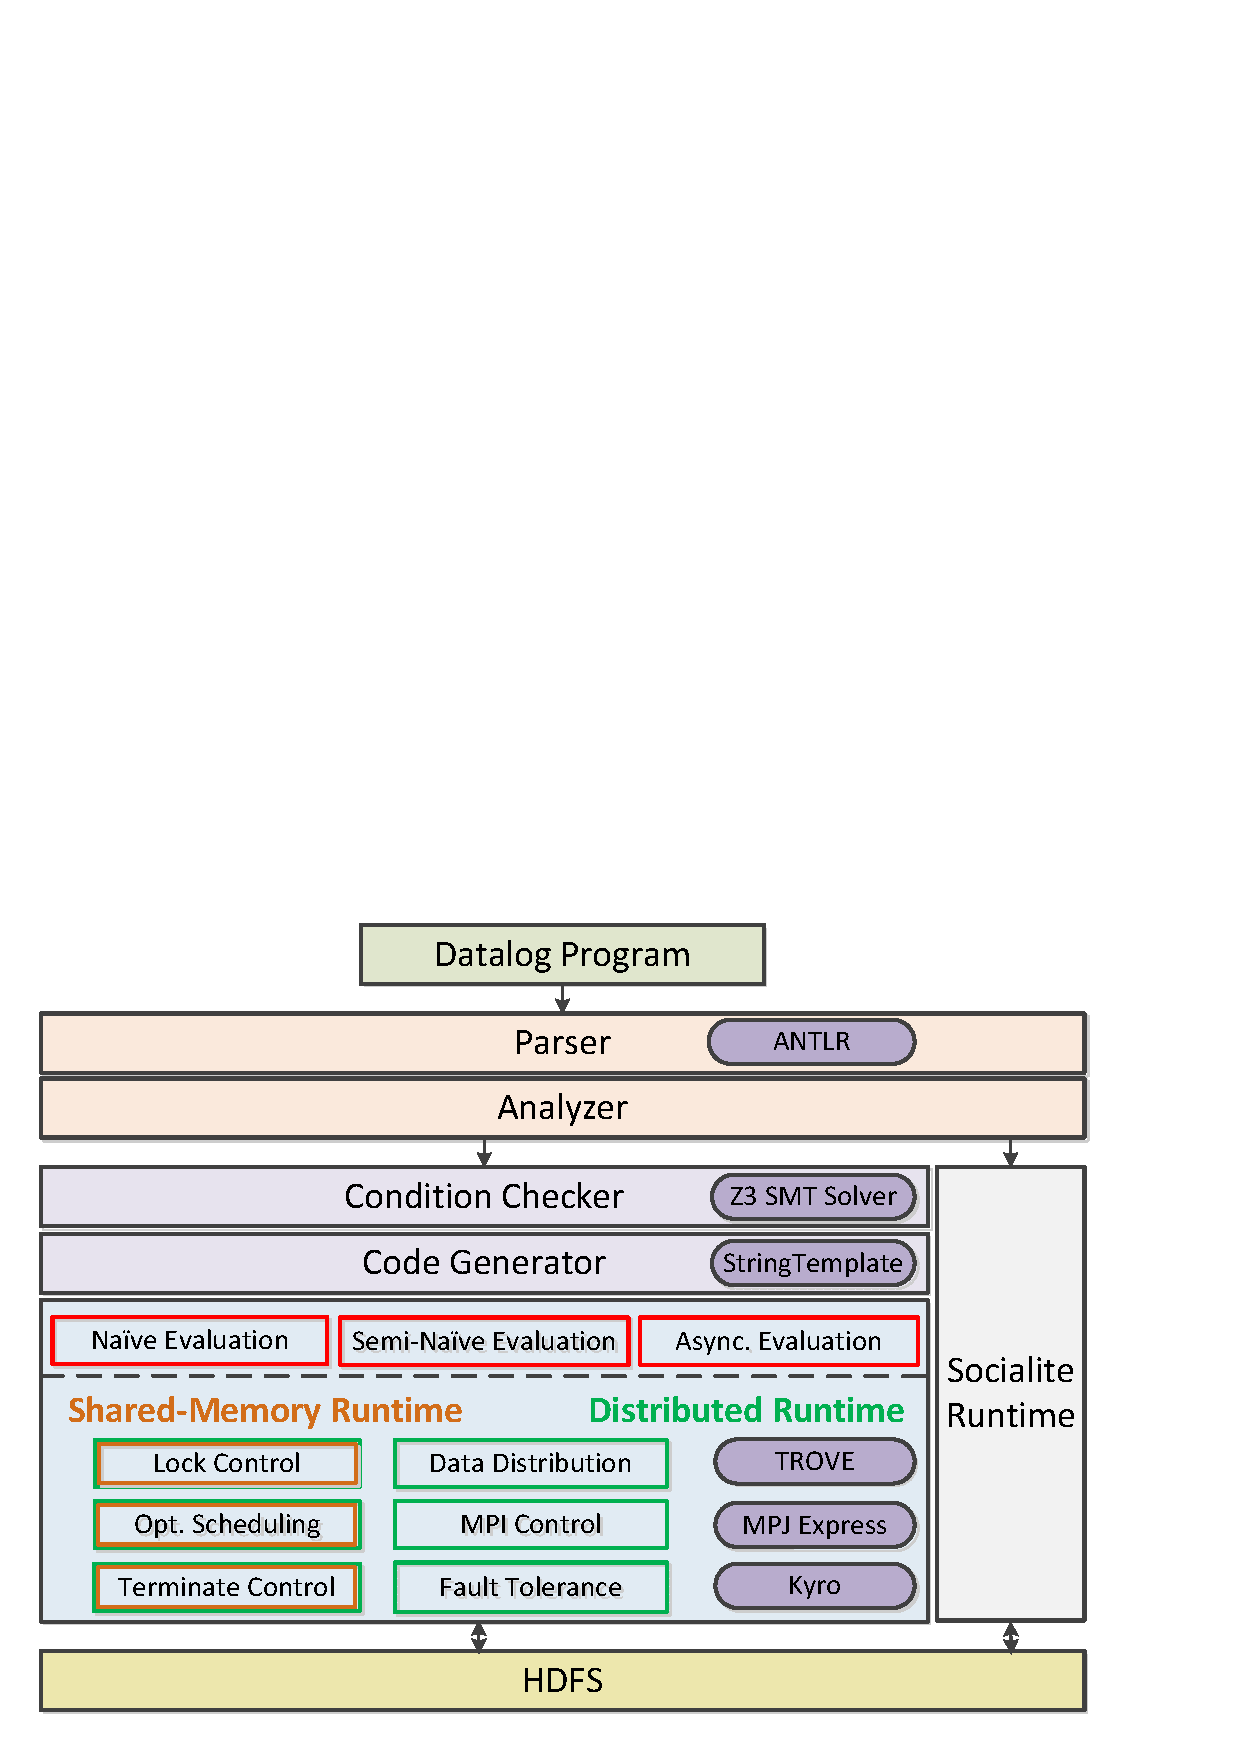
\includegraphics[width=3.2in]{fig/overview2}
  \vspace{-0.1in}
  \caption{A3Log overview}
  \label{fig:overview}
  \vspace{-0.2in}
\end{figure}

A3Log is implemented using Java and contains several components as shown in Fig. \ref{fig:overview}. The \textbf{Parser} parses user's Datalog program into an abstract syntax tree (AST) by using ANTLR \cite{antlr}. The \textbf{Analyzer} traverses the AST to performs syntactic and semantic analysis, identifies the recursive rule, and analyzes the aggregate operation $g$ and non-aggregate operation $f$. If the program is a recursive program, it will be further processed by our system, otherwise it will be executed by the Socialite runtime engine \cite{Lam:2013:SDE:2510649.2511289,Seo:2013:DSD:2556549.2556572}. Given the $f$ and $g$ operations retrieved by the Analyzer, the \textbf{Condition Checker} relies on Z3 SMT Solver \cite{DeMoura:2008:ZES:1792734.1792766,z3} to verify the conditions and automatically chooses the appropriate evaluation technique. The \textbf{Code Generator} provides a series of code templates for generating the share-memory runtime code and distributed runtime code, where we use StringTemplate \cite{stringtemplate} to generate source code. Then, the recursive program will be executed by our execution engine (Sec. \ref{sec:system:runtime}). A3Log provides both \textbf{Shared-Memory Runtime Engine} and \textbf{Distributed Runtime Engine}. The shared-memory runtime and distributed runtime share several functionalities, including lock control, scheduling, termination check. The distributed runtime additionally supports data distribution, MPI control, and fault tolerance. We use TROVE \cite{trove} for high performance container operations which are frequently used due to our key table structure, use openmpi \cite{mpich} for  communication, and use ProtoStuff \cite{Protostuff} for efficient serialization and deserialization. As implemented in Socialite, A3Log also relies on HDFS to store data and to checkpoint intermediate computation state.

\subsection{Datalog and Extension}
\label{sec:system:datalog}

A Datalog program is a set of rules. A \emph{rule} \texttt{r} has the form $h\leftarrow b_1,\ldots,b_n$, where $h$ is the \emph{head} and $b_1,\ldots,b_n$ is the \emph{body}. The comma separating literals in a body is a logical conjunction (AND). $h$ and $b_i$ can be with the form $p_i(t_1,\ldots,t_j)$ where $p_i$ is a \emph{predicate} and $t_1,\ldots,t_j$ are terms which can be \emph{constants}, \emph{variables} or \emph{functions}. For example, the Datalog program for PATH computation can be written as follows.
%The data associated with abstract predicate is referred to as \emph{fact}.
\begin{comment}
\begin{verbatim}
Program 1. Single Source Shortest Path
\end{verbatim}
\vspace{-0.1in}
\small
\begin{lstlisting}
r1. sssp(X,$d$)$\leftarrow$ X=1,$d=0$.
r2. sssp(Y,min[$d$])$\leftarrow$ sssp(X,$d1$),edge(X,Y,$d2$),
		     $d=d1+d2$,sssp(Y,$d$).
\end{lstlisting}
\normalsize

In Program 1, rule \texttt{r1} initializes the predicate \texttt{sssp} by specifying the source node $X=1$ and the shortest distance from source as $d=0$. \texttt{r2} is a recursive rule since it has the \texttt{sssp} predicate in both its head and body. \texttt{r2} will recursively produce \texttt{sssp} fact by joining the old \texttt{sssp} and \texttt{edge}. If there is a path from source to $X$ of length $d_1$ and an edge from $X$ to $Y$ of length $d_2$, there is a path from source to $Y$ with length $d=d_1+d_2$. If there is already a path to $Y$ found before, it should be also considered. Hence, the shortest distance from source to $Y$ is updated by the minimum of these possible distances, i.e., min$[d]$. The recursion will terminate as soon as no shortest distance is updated.
\end{comment}
 \begin{verbatim}
 Program 1. Computing Paths in a DAG
 \end{verbatim}\vspace{-0.1in}\small
 \begin{lstlisting}
 r1. cpaths(X,Y,$c$) $\leftarrow$ edge(X,Y), $c=1$.
 r2. cpaths(X,Y,[$c$]) $\leftarrow$ cpaths(X,Z,$c$),
                          edges(Z,Y),
                          cpaths(X,Y,$c$).
 \end{lstlisting}
 \normalsize
 
 Program 4 counts the paths between pairs of vertices in an acyclic graph. \texttt{r1} counts each edge as one path between its vertices. In \texttt{r2}, any \texttt{edge(Z,Y)} that extends from a computed path count \texttt{cpath(X,Z,$c$)} establishes $c$ distinct paths from \texttt{X} to \texttt{Y} through \texttt{Z}.
 
Originally, the Datalog program terminates when no new fact can be found. However, some programs will never stop since it continuously produces ``tiny'' facts. For example, the PageRank computation will continuously update the PageRank scores even though the changes are less and less. In order to help users express more termination conditions, we allow users to specify the termination conditions using aggregations.


\begin{verbatim}
Program 2 PageRank
\end{verbatim}
\vspace{-0.1in}
\small
\begin{lstlisting}
r1. degree(X,count[Y])$\leftarrow$ edge(X,Y).
r2. rank(X,$r$) $\leftarrow$ node(X),$r=1$.
r3. rank(Y,sum[$r$]+0.15) $\leftarrow$ rank(X,$r1$),edge(X,Y),
			degree(X,$d$),$r=0.85\cdot r1/d$,
			[sum$[\Delta r]\leq 0.001$].
\end{lstlisting}
\normalsize

In Program 2, we show the Datalog program for PageRank. \texttt{r1} computes the node degrees based on the edge data. \texttt{r2} initializes the predicate \texttt{rank} by specifying all the nodes' ranking scores as a constant 1. \texttt{r3} is a recursive rule that updates the predicate \texttt{rank}. We allow users to specify the terminate conditions in $[\ldots]$ by using different aggregate operations. In this program, the PageRank computation will terminate when the sum of ranking score differences of two continuous recursion results is less than or equal to 0.001.

Besides PATH and PageRank, we list 11 more example Datalog programs that can be executed asynchronously in the technical report \cite{fullversion}. These examples cover a wide range of applications, including graph analytics, data mining, machine learning, and HPC.

\subsection{Condition Checker}
\label{sec:system:condition}

\begin{figure}[!t]
    \centering
  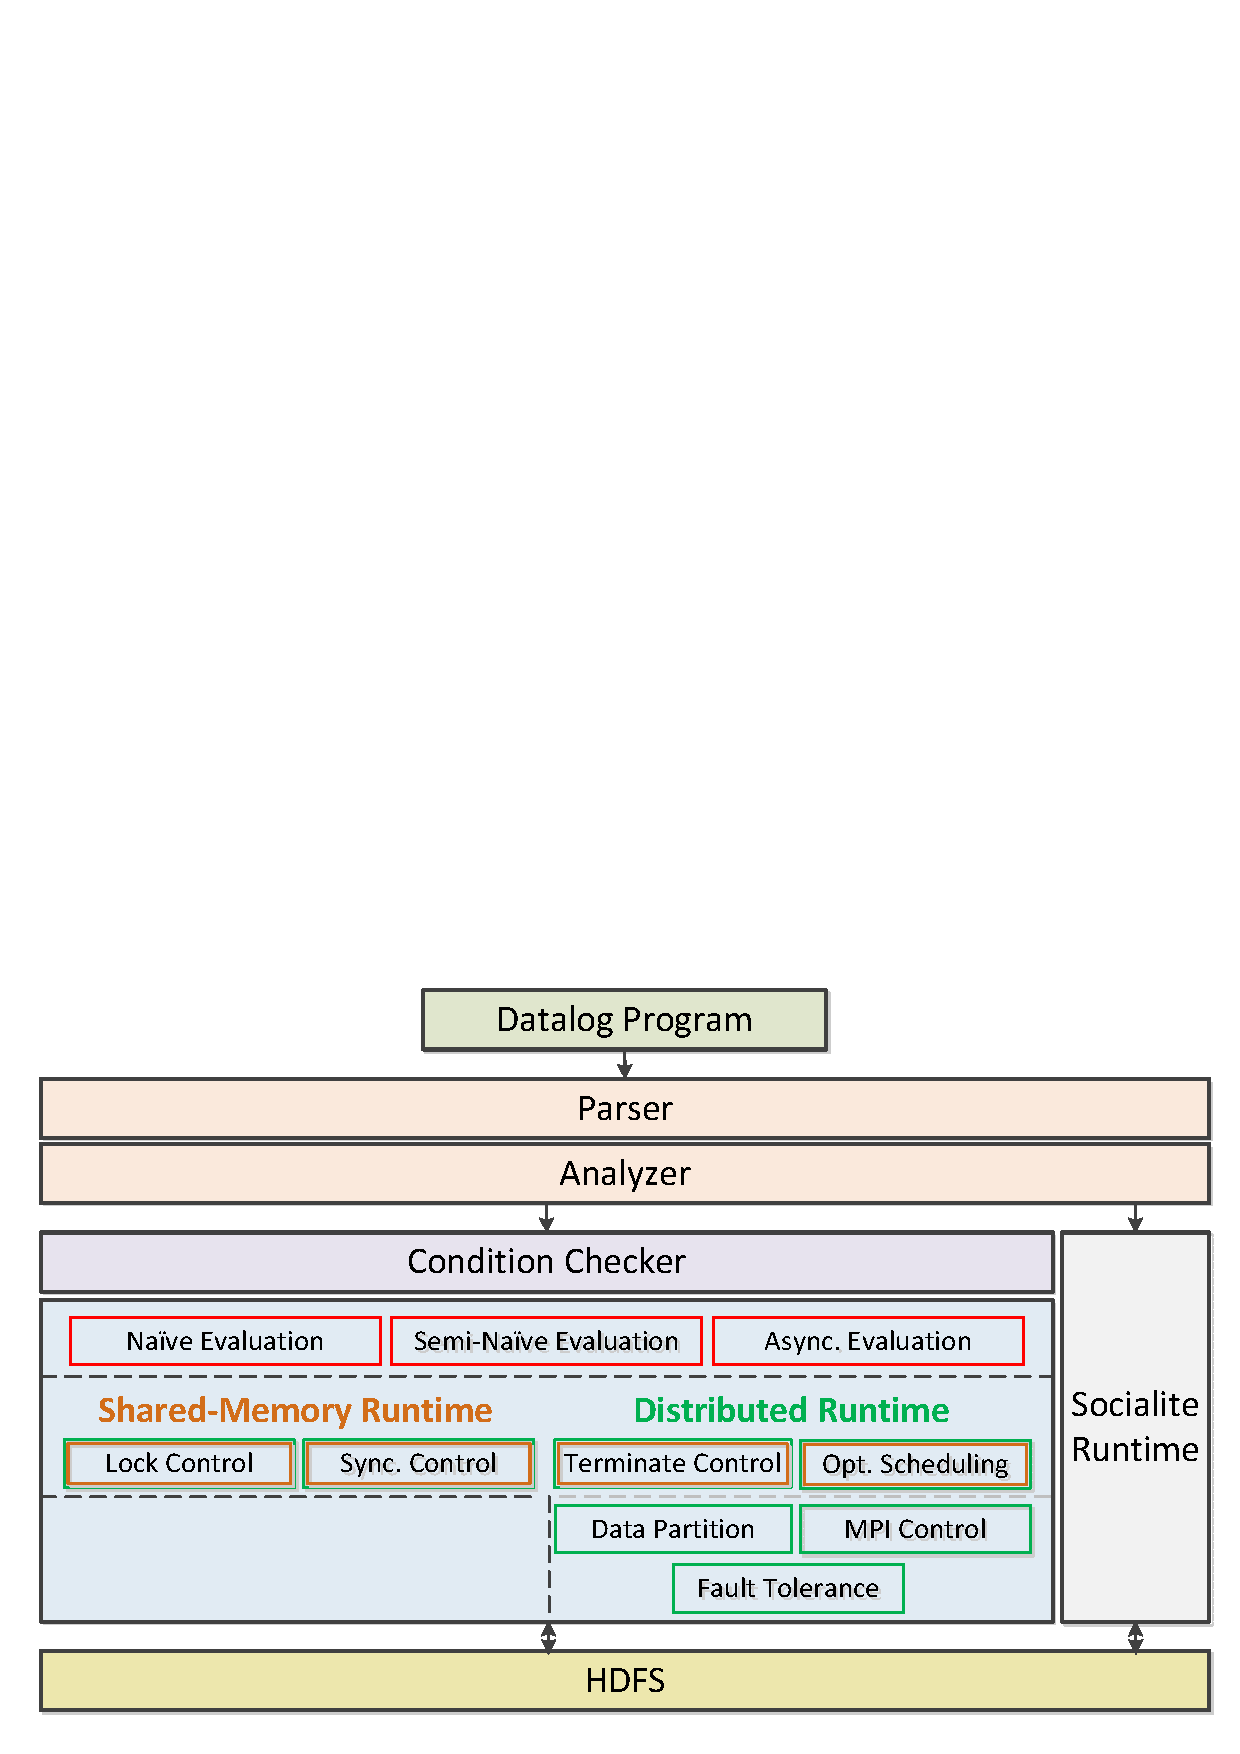
\includegraphics[width=2.8in]{fig/flow}
  \vspace{-0.1in}
  \caption{Condition checking flow chart}
  \label{fig:flow}
  \vspace{-0.2in}
\end{figure}

A3Log is able to automatically verify the conditions for asynchronous aggregation and accordingly selects the appropriate optimization technique according to the satisfiable conditions. The $g$ operation is identified as the update operation in the recursive rule's head predicate, e.g., min[$d$] in SSSP and sum[$r$]+0.15 in PageRank where [$d$] and [$r$] are the inputs, respectively. The $f$ operation is identified as the computation in the recursive rule's certain body predicate that updates the input variables of $g$ operation, e.g., $d=d1+d2$ in SSSP and $r=0.85\cdot r1/d$ in PageRank. The input variable of $f$ operation is the variable that appears in the recursive predicate, e.g., $d1$ in \texttt{sssp(X,$d1$)} and $r1$ in \texttt{rank(X,$r1$)}.

There are two techniques for executing recursive Datalog programs. The first is \emph{\textbf{Naive Evaluation}}. For instance, in Program 1, the recursive rule \texttt{r2} will be repeatedly evaluated. The \texttt{edge} facts keep being joined with the \texttt{sssp} facts discovered so far in each iteration, until no new fact is produced. This approach will inefficiently re-produce known facts in every iteration. To address this inefficiency issue, the \emph{\textbf{Semi-Naive Evaluation}} for recursive programs with aggregation was proposed \cite{Lam:2013:SDE:2510649.2511289,Wang:2015:AFR:2824032.2824052}, which is efficient and produces no duplicates. However, the semi-naive evaluation requires the program to be set-containment monotonic in order to guarantee the correctness. This is the same as the monotonizability condition that we have defined in Theorem \ref{th:monotone}. Therefore, as long as the program satisfies monotonizability condition or can be converted to be monotonic according to Theorem \ref{th:convert}, it can be executed with semi-naive evaluation. Furthermore, we propose \emph{\textbf{asynchronous evaluation}} as a yet another optimization technique, which allows asynchronous aggregation. We provide the sufficient conditions for asynchronous aggregation in Theorem \ref{th:async}. The prerequisite for asynchronous aggregation is the monotonic condition. Asynchronous evaluation is possible only when the recursive program is monotonic and satisfies order independent condition.

Condition Checker first translates the $f$ and $g$ operations into Z3 \cite{DeMoura:2008:ZES:1792734.1792766} satisfiability formulas (see Sec. \ref{sec:async:autoasync}). By applying $f$ and $g$ to the built-in condition checking templates, the Z3 SMT olver will answer satisfiable, unsatisfiable, or unknown. Following the condition checking flow as shown in Fig. \ref{fig:flow}, our system can automatically select the appropriate evaluation technique.

\subsection{Key Data Structure: AsyncTable}
\label{sec:system:data}

Before launching the recursive computation, the key table structure, AsyncTable, should be first prepared. AsyncTable maintains the computation states, which are initialized based on user's Datalog program and keeps being updated during the whole recursive computation process.

\begin{figure}[!t]
    \centering
  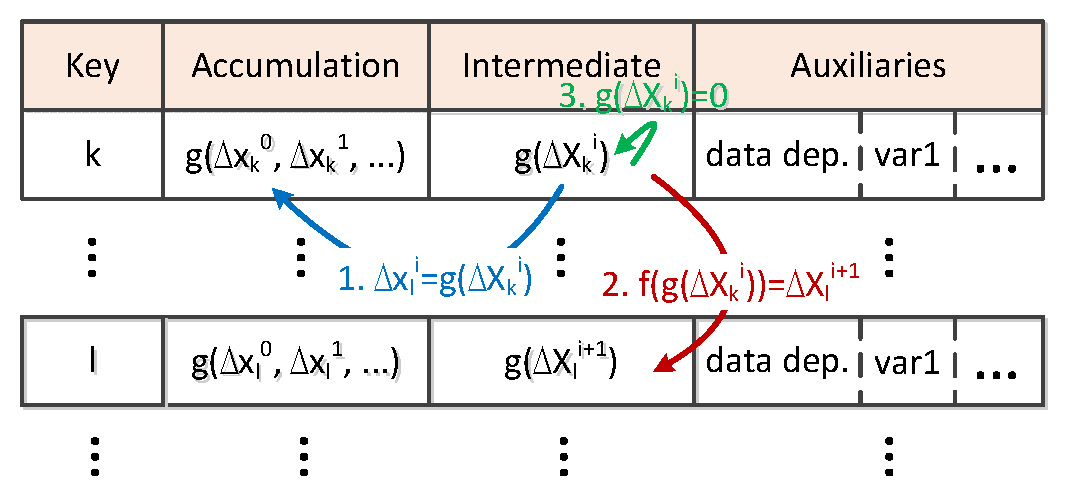
\includegraphics[width=3.2in]{fig/asynctable}
  \vspace{-0.0in}
  \caption{AsyncTable update}
  \label{fig:asynctable}
  \vspace{-0.0in}
\end{figure}


\noindent\textbf{AsyncTable Design}
As shown in Fig. \ref{fig:asynctable}, the AsyncTable contains several columns. The main key column and accumulation column store the result key-value pairs. The main key entries index the table. The accumulation column entry monotonically aggregates the intermediate results and maintains $g(\Delta x^0,\Delta x^1,\ldots)$. The accumulative property of $g$ operation makes it possible to use a single column to maintain all the intermediate results,i.e. The intermediate column entry stores the temporary aggregation results $g(\Delta X^k)$ which will be used to generate future intermediate results by applying $f$ operation. The auxiliary columns store the data which might be used by the $f$ or $g$ operation, e.g., outgoing neighbors set in PATH and the node degree value in PageRank. The accumulation column entries and intermediate column entries are volatile, which maintain the computation states and keep being updated during the computation, while the other column entries are fixed after initialization. The AsyncTable is sharded for parallel processing. Each shard contains a number of rows and is assigned to a compute thread or placed on a distributed worker machine.

\noindent\textbf{AsyncTable Initialization}
The AsyncTable is initialized according to user's program. The recursive rule head contains the main key and accumulation column's information. For example in PATH, the main key column entries are initialized with the node pairs ids. The accumulation column is initialized with the identity element \textbf{0} w.r.t $g$, e.g., SUM in PATH. The intermediate column is initialized in terms of the non-recursive rule \texttt{r1}, i.e., 1 if there is an edge between the node pair and 0 for other nodes. The auxiliary data dependency column is identified as the rule body predicate that describes the relationship between main keys, e.g., \texttt{edge(Z,Y)}. The auxiliary variable column entries can be identified as the joined results between rule body predicates, e.g., the degree information \texttt{d} in PageRank.

A few additional facts should be noticed: 1) It is possible that two or more items are identified as the main key  2) The AsyncTable size can be dynamic rather than fixed due to the continuously inserted new rows 3) The recursive program can be composed of more than one interdependent rules, which can be reduced to one rule.

\subsection{Execution Runtime Engine}
\label{sec:system:runtime}

\begin{figure}[!t]
    \centering
  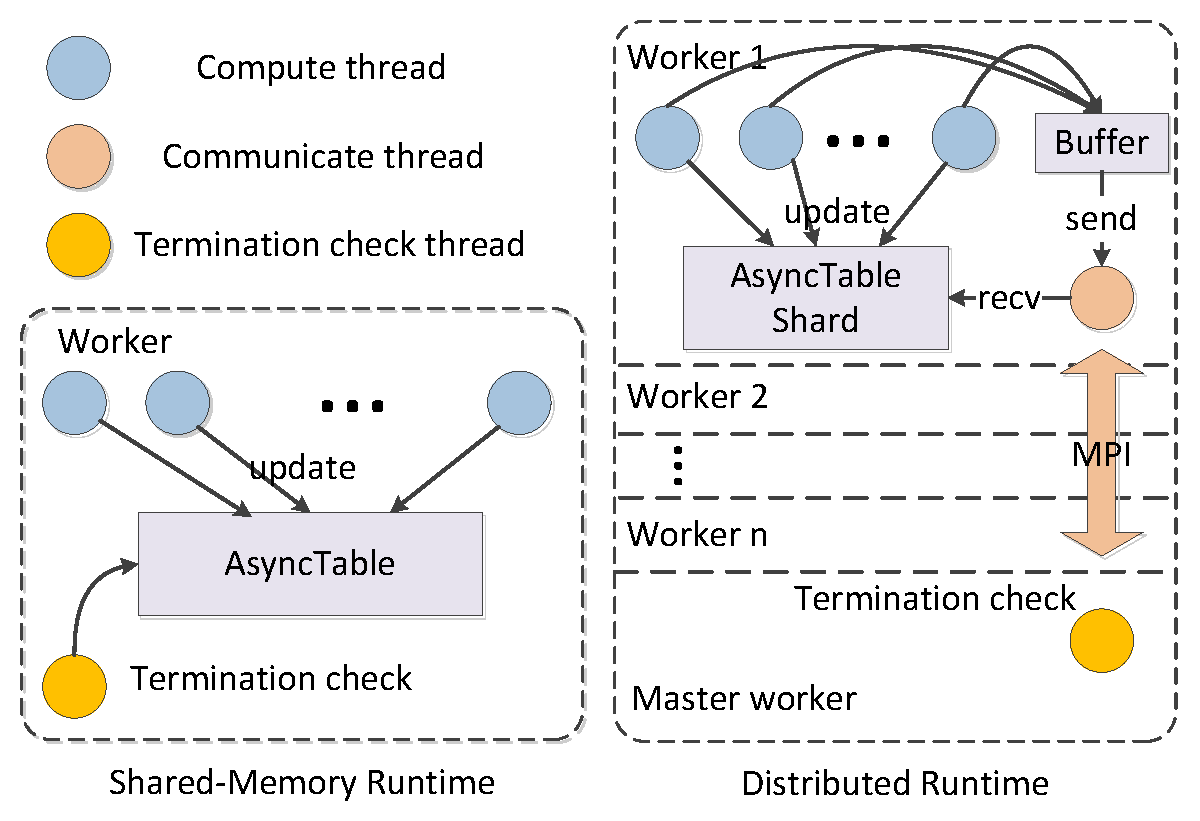
\includegraphics[width=2.9in]{fig/runtime}
  \vspace{-0.0in}
  \caption{Execution Runtime Engine}
  \label{fig:runtime}
  \vspace{-0.1in}
\end{figure}

\noindent\textbf{Overall Architecure}
A3Log provides both shared-memory runtime engine and distributed runtime engine. Fig.\ref{fig:runtime} shows the overall structure. The shared-memory runtime has a simple design. A number of compute threads are created to update the AsyncTable in parallel, and a termination check thread is running separately to check the stop condition. The distributed runtime contains a number of workers and a master worker. Each worker creates a number of compute threads to update the local AsyncTable shard. A communicate thread tackles the remote update. We adopt a send buffer design to control the overhead of frequent communications. The master worker creates a termination check thread to globally check stop condition periodically.


\noindent\textbf{Concurrency Control}
The accumulation column entries and intermediate column entries keep being updated during computation. Specifically, an intermediate column entry is read to update the same row's accumulation column entry (by operation 1 in Fig.\ref{fig:asynctable}) and to update other rows' intermediate column entries (by operation 2 in Fig.\ref{fig:asynctable}), and is reset as \textbf{0} (by operation 3 in Fig.\ref{fig:asynctable}). The reset operation is essential to make result correct, without which the same intermediate result would be redundantly accumulated. These three operations have to be \emph{atomic} according to the definition of accumulated recursive program (Definition \ref{eq:accumasync}). However, an intermediate column entry can be read and written concurrently by multiple threads or multiple workers, which leads to potential consistency problem. In our shared-memory runtime, we use \emph{optimistic} lock to avoid read-write conflicts. In distributed runtime, the consistency problem will happen in the send buffer, which maintains the remote updates. The optimistic lock does not work well since the communicate thread is required to serialize the whole buffer for efficiency and the lock granularity becomes too coarse to result in too many aborts. We employ MVCC (multi-version concurrency control) to address this problem. Specifically, we adopt a double-version design of the send buffer, which serves the compute threads and communicate thread alternatively.


\noindent\textbf{Scheduling}
When executed in synchronous module,There is no necessary or chance to schedule the computing.But in asynchronous module.The clever scheduling of aggregate operations has the potential of accelerating the convergence of recursive computations.The scheduling should be performed by evaluating the intermediate aggregation result (intermediate column entries in AsyncTable). The top intermediate column entries (in the partial order defined by $g$) should be scheduled. Since the intermediate column entries keep being updated, the top entries should be evaluated frequently. For the sake of reducing scheuduling cost, we utilize the sampling technique \cite{Zhang:2011:PDF:2038916.2038929} to approximately obtain the top $N\%$ entries. The scheduling is even more costly in distributed environment. Rather than global scheduling, local scheduling in each worker is preferred.
%The portion ($N\%$) of entries to be scheduled balances the tradeoff between the optimal scheduling benefit and the sorting cost. We will empirically study the effect of $N\%$ in Sec. \ref{sec:expr:schedle}.

\noindent\textbf{Termination Check}
The termination condition might rely on aggregation of either the accumulation column entries or the intermediate column entries. The aggregation is evaluated by the termination check thread without disturbing the compute threads. While in distributed runtime, each worker will report their local aggregation results to the master, where the global termination check thread determines whether to stop by evaluating the global aggregation result. Note that, there is no iteration's conception in asynchronous aggregation, so we have to check the termination condition every other period of time rather than every other iteration.

\noindent\textbf{Fault Tolerance}
For large scale operations that involve many machines for a substantial amount of time, it is also important to provide fault tolerance support. A3Log relies on Socialite's fault tolerance scheme \cite{Seo:2013:DSD:2556549.2556572}. The intermediate computation states are checkpointed occasionally on HDFS and restorable as needed. If one or more workers fail, the intermediate states are restored from the latest checkpoint and the evaluation is resumed from that point.


\section{Performance Evaluation}
\label{sec:expr}
\begin{comment}
\begin{table*}[!t]
	%\vspace{-0.1in}
	\caption{The Result of some Common Algorithms }
	\hspace{-0.15in}
	\vspace{0.0in}
	\label{tab:resut}
	\centering
	\small
	\begin{tabular}{c|c|c|c|c|c|c|c}
		%	\hline
		%		\multirow{2}{*}{\textbf{Dataset}} & \multirow{2}{*}{\tabincell{c}{\textbf{Nodes}}} & \multirow{2}{*}{\tabincell{c}{\textbf{Edges}}} & \multirow{2}{*}{\tabincell{c}{\textbf{Graph}\\ \textbf{type}}} & \multirow{2}{*}{\tabincell{c}{\textbf{$d$}}}& \multirow{2}{*}{\tabincell{c}{\textbf{$e$}}} & \multicolumn{3}{|c}{\textbf{SSSP}} & \multicolumn{3}{|c}{\textbf{PageRank}} \\
		%		\cline{7-12}
		%		&  & & & & & \textbf{Sync.} & \textbf{Async.} & \footnotesize{\textbf{Speedup}} & \textbf{Sync.} & \textbf{Async.} & \footnotesize{\textbf{Speedup}}\\
		\hline\hline
		{\textbf{Algorithm}} &
		{\textbf{$g$}} &
		{\textbf{$f$:(broadcast, self)}} &
		{\textbf{Monot}} &
		{\textbf{Commu}} &
		{\textbf{Accumu}} &
		{\textbf{OrderInd}} &
		{\textbf{Conver}}\\
		\hline
		\textbf{Pagerank} & $sum(\centerdot)$ &($(1-c)*x$), $0.15$   &$\times$ & $\surd$ & $\times$  & - &$\surd$\\
		\hline
		\textbf{SSSP} & $min(\centerdot)$ & ($x+w$), $x$ &$\surd$ & $\surd$& $\surd$ & $\surd$ & -\\
		\hline
		\textbf{CC} & $min(\centerdot)$& ($x$), $x$ & $\surd$ & $\surd$ & $\surd$ & $\surd$ & -\\
		\hline
		\textbf{PATH} & $sum(\centerdot)$ &$(x)$, $x$& $\surd$ &$\surd$& $\surd$ & $\surd$ & -\\
		\hline
		\textbf{MAX PRO PATH} & $max(\centerdot)$ &  send$(p_1\& p_2) p=p_1*p_2$, p & $\surd$ & $\surd$ & $\surd$ & $\surd$ & -\\
		\hline
		\textbf{COST} & $sum(\centerdot)$&$(x*n)$, $x$ & $\surd$ & $\surd$ & $\surd$ & $\surd$ & -\\
		\hline
		\textbf{Viterbi} & $max(\centerdot)$ & $L=L_1*L_2*L_3$, $nothing$ & $\times$ & $\surd$ &  $\surd$ &  - &$\times$\\
		\hline
		\textbf{PARTY} & $count(\centerdot)$&$((x)\&(N>3))$,x & $\surd$ & $\surd$ & $\surd$ & $\surd$ & -\\
		\hline
		\textbf{Galaxy evolution} & $count(\centerdot)$ &$pract(gid1\& gid2)$, gid& $\surd$ & $\surd$ & $\surd$ & $\surd$ & -\\
		\hline
		\textbf{Belief propagation} & $sum(\centerdot)$ &$w*x*h$, $nothing$ & $\times$ & $\surd$ & $\surd$ & - & $\surd$\\
		\hline
		\textbf{Simrank} & $sum(\centerdot)$& $c/(d_1*d_2)*x$, $nothing$ & $\times$ &  $\surd$ &  $\surd$ & - & $\surd$\\
		\hline
		\textbf{Jacobi Method} &$sum(\centerdot)$ &$-a_{ij}/a_{ii}*x$, $c$& $\times$ & $\surd$  & $\times$ & - & $\surd$\\
		\hline
		\hline
	\end{tabular}
	\vspace{-0.1in}
\end{table*}
First, we exhibit conditions satisfiability of some common algorithms.
We empirically evaluate A3Log on Amazon EC2. We will show the comparison results with other systems, with different algorithms, and with different datasets.
\subsection{Result of Condition Checker}


In this section, we test more algorithms to check the asynchronous conditions. We list $f$ and $g$ operations and each property of each algorithm. As shown in table \ref{tab:resut}, SSSP, CC, DAG, PATH, COST and Galaxy evolution algorithm  can be correctly asynchonized directly. Belief Propagation,pagerank, Jacobi Method and Simrank doesn't satisfy the monotonic condition. While all these five algorithm can be converted to accumulative recursive aggregation model and executed asynchronously. Viterbi algorithm  satisfy neither the monotonic condition nor the convertibility condition.
\end{comment}
\subsection{Comparison to Other Systems}
\label{sec:expr:othersystems}

\Paragraph{Competitors}
A3Log is compared with three state-of-the-art Datalog frameworks. \textbf{SociaLite} \cite{Lam:2013:SDE:2510649.2511289,Seo:2013:DSD:2556549.2556572} is a Datalog implementation for social network analysis. \textbf{Myria} \cite{Halperin:2014:DMB:2588555.2594530,Wang:2015:AFR:2824032.2824052} supports Datalog asynchronous evaluation. And \textbf{BigDatalog}\cite{Shkapsky:2016:BDA:2882903.2915229} a Datalog implementation based on spark. All these three framework support monotonic aggregation inside recursion.
%\textbf{GraphLab} \cite{Low:2012:DGF:2212351.2212354} is a graph-based parallel/distributed engine supporting asynchronous iteration. \textbf{Maiter} \cite{maiter} supports delta-based accumulative iterative computation which can be executed asynchronously.
All these systems are configured with their default parameters.
%Myria, GraphLab, and Maiter are configured to run with asynchronous model unless particularly mentioned.
 The runtime results are the execution time excluding data loading time, and each is a mean of three runs.

\Paragraph{Algorithms and Dataset}
We compare A3Log with other systems in the context of three algorithms, including SSSP, Connected Components(Asynchronizable)and PageRank(convertible). These three algorithms are all supported by these systems\footnote{Since BigDatalog doesn't support monotonic aggregate function $msum$ and $mcount$, so it is hard to express PageRank computation with BigDatalog. So we use GraphX as a instead for PageRank experiment.}.
% For SSSP and CC, the computations terminate as soon as no new update is found. For PageRank in A3Log and Maiter, which has no notion of iterations, the computation terminates when the sum of difference to the theoretical convergence point \cite{Zhang:2011:PDF:2038916.2038929} is less than $10^{-3}$, based on which we know the number of iterations that is required to reach the same point (42 iterations) \cite{Zhang:2011:PDF:2038916.2038929}. Socialite and Myria (Myria does not support asynchronous PageRank) are set to run 42 iterations. GraphLab terminates after the PageRank value of every vertex changes by less than a user-specified threshold $\epsilon$ between two consecutive executions of that vertex. These algorithms are performed on a large graph dataset ClueWeb09 \cite{clueweb}. In order to finish the experiments in a reasonable time, we truncate the original dataset into a smaller ClueWeb20M dataset with 20,000,000 nodes, 243,063,334 edges, and 3.8GB size. Since ClueWeb is an unweighted graph, we assign a random weight to each edge for SSSP computation.
\begin{table}[!t]
	%\vspace{-0.1in}
	\caption{Parameter of RealWorld Graph }
	\hspace{-0.15in}
	\vspace{0.0in}
	\label{tab:Dataset}
	\centering
	\small
	\begin{tabular}{c|c|c|c}
		\hline\hline
		{\textbf{Name}} &
		{\textbf{Vertices}} &
		{\textbf{Edges}} &
		{\textbf{Source}} \\
		\hline
		{\textbf{Flickr}} & 2,302,925 &33,140,017   & \cite{mislove-2008-flickr}\\
		\hline
		{\textbf{LiveJournal}} & 4,847,571 & 68,475,391 &\cite{livejournal}\\
		\hline
		{\textbf{Orkut}} &3,072,441& 117,184,899 & \cite{mislove-2007-socialnetworks} \\
		\hline
		{\textbf{culeweb09}} & 20,000,000 & 243,063,334 &\cite{clueweb}\\		\hline
		{\textbf{Wiki-link}} & 12,150,976 &378,142,420&\cite{wikilinks} \\
		\hline
		{\textbf{arabic-2005}} & 22,744,080 & 639,999,458 &\cite{arabic-2005}\\		\hline
		\hline
	\end{tabular}
	\vspace{-0.1in}
	
\end{table}
We perform all the three algorithm on all datasets in Table \ref{tab:Dataset}.
\begin{comment}
\begin{figure}[!t]
	\vspace{0.08in}
	\centering
	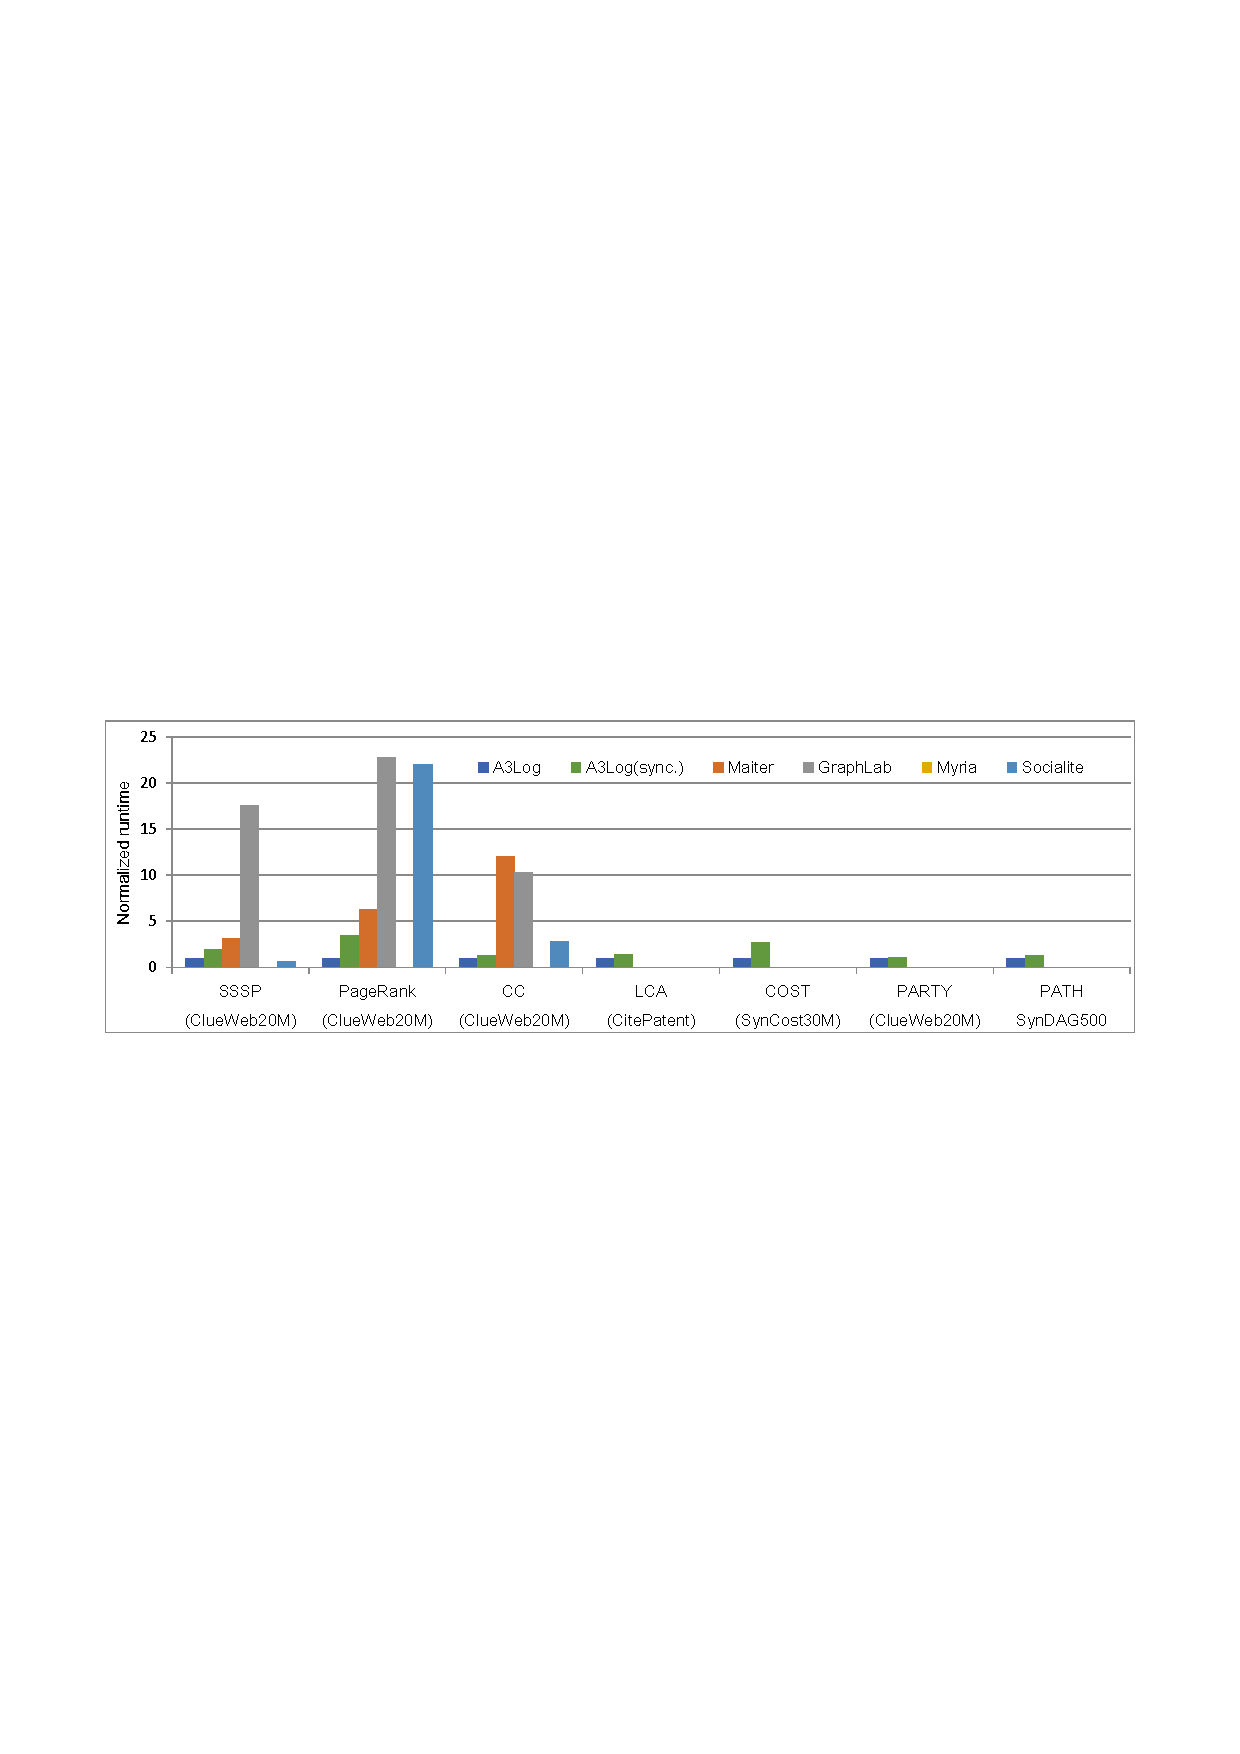
\includegraphics[width=3in]{fig/single-result}
	\vspace{-0.1in}
	\caption{Performance comparison with other systems (many-core environment)}
	\label{fig:single-result}
	\vspace{-0.2in}
\end{figure}
\end{comment}



%In the shared-memory experiment, we run all the systems on an r3.8xlarge EC2 instance with 32 vCPUs and 244GB memory. We configured all these systems with 32 threads. The normalized runtime results. In general, A3Log outperforms all the competitors. For the PageRank computation, A3Log achieves 22.8X speedup over GraphLab, 22X speedup over Socialite, 6X speedup over Maiter, and much more speedup over Myria\footnote{The runtime results of Myria may be wrong because they are all unexpected long, say 135 times longer for PageRank and 321 times longer for SSSP than A3Log. We are contacting with Myria authors to fix it but cannot find the problem before the submission.} are shown in Fig. \ref{fig:single-result}. There is an exception for SSSP computation. Socialite is 1.6X faster than A3Log. This may be due to their \emph{prioritization} optimization, which is similar to our scheduling technique that leads to Dijkstra algorithm.

\begin{figure*}[!t]
	\vspace{1in}
	\centering
	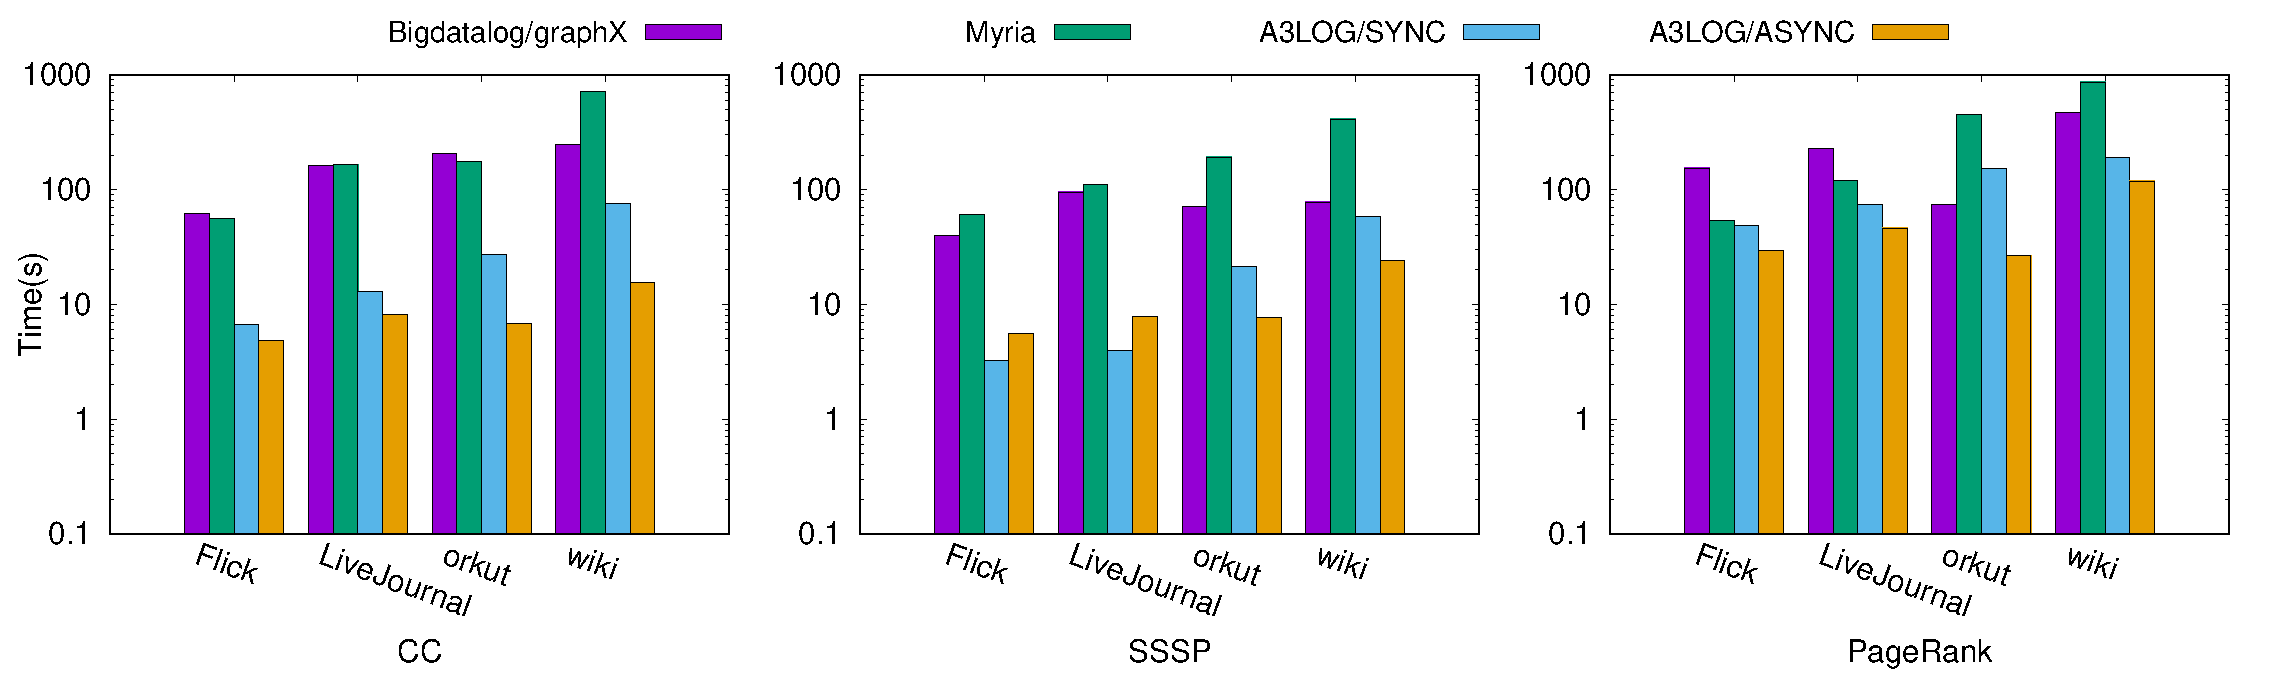
\includegraphics[width=6.6in]{figuration/compare.eps}
	\vspace{-0.1in}
	\caption{Performance comparison with other systems (distributed environment)}
	\label{fig:dist-result}
\end{figure*}
In the distributed comparsion we deploy all the systems on an Aliyun ECS cluster with
16 ecs.r5.xlarge ECS instances, each with 4 vCPUs and 32GB memory. The network bandwidth between instance workers is  1.5Gbps/s. We configured all these systems with 4 threads for each worker. Myria was configured with one instance of Myria and PostgreSQL. For bigdatalog, we evaluate with one partition per available CPU core, and configured according to\cite{Shkapsky:2016:BDA:2882903.2915229}. For asynchronous A3log we set the Message buffer size to 500, 1000, 2000 in turn and reserve the best one. Runtime results are shown in Fig.\ref{fig:dist-result}. 

\textbf{Connected component} A3log outperform all these three competitor with asynchronous processing. Socialite outperforms the synchronous version of A3log on Orkut datasets. Socialite has run out of memory on wiki-link datasets.

\textbf{SSSP} A3log outperforms all these three competior with asynchronous version .Socialite outperforms the synchronous version of A3log on Orkut datasets. And further asynchronous processing doesn't beat synchronous version in Flickr and LiveJournal, But the later experiments show that our optimization technology performs quite well on big datasets.

\textbf{PageRank}
For PageRank algorithm, A3log outperforms all the other system except Bigdatalog/GraphX on Orkut dataset with synchronous processing. Asynchronous A3log shows much better performace than GraphX. And without the support of seminaive technology, socialite is no longer competitive.


%GraphLab and Socialite on PageRank computation. The synchronous version of GraphLab performs much better than asynchronous Graph-Lab, which is due to its costly distributed locking \cite{Han:2015:GUB:2777598.2777604,Low:2012:DGF:2212351.2212354}.
%Socialite performs SSSP only a little faster almost negligible.The distributed Myria runs unexpected long without returning results, say 9 hours for PageRank and did not return. The performance of A3Log and Maiter is comparable on these two applications,and Maiter performs pagerank even faster.The reason why A3Log does not show significant better performance in distributed environment is because of the expensive communication and serialization overhead.The performance of communicate and serialize components implemented in java unmatched that of C/C++ implementation.
%\begin{comment}
\subsection{Effects of Adaptive Message Buffer}
\label{sec:expr:AMBuffer}
In this section, we evaluate the effectness of adaptive message buffer strategy described in \ref{fig:intro} on the Same three application and \emph{What is the cost of each part}\cite{7113340}. To evaluate the performance with other optimization technology, we also implement priority scheduling technology. We perform the previous three algorithm on four dataset, and for the \textbf{COST} algorithm we synthetically generate a hierarchical (tree-like) dataset with 64000000 tree nodes.

\Paragraph{Overall evaluation}
\begin{figure*}[!t]
	\vspace{0.0in}
	\centering
	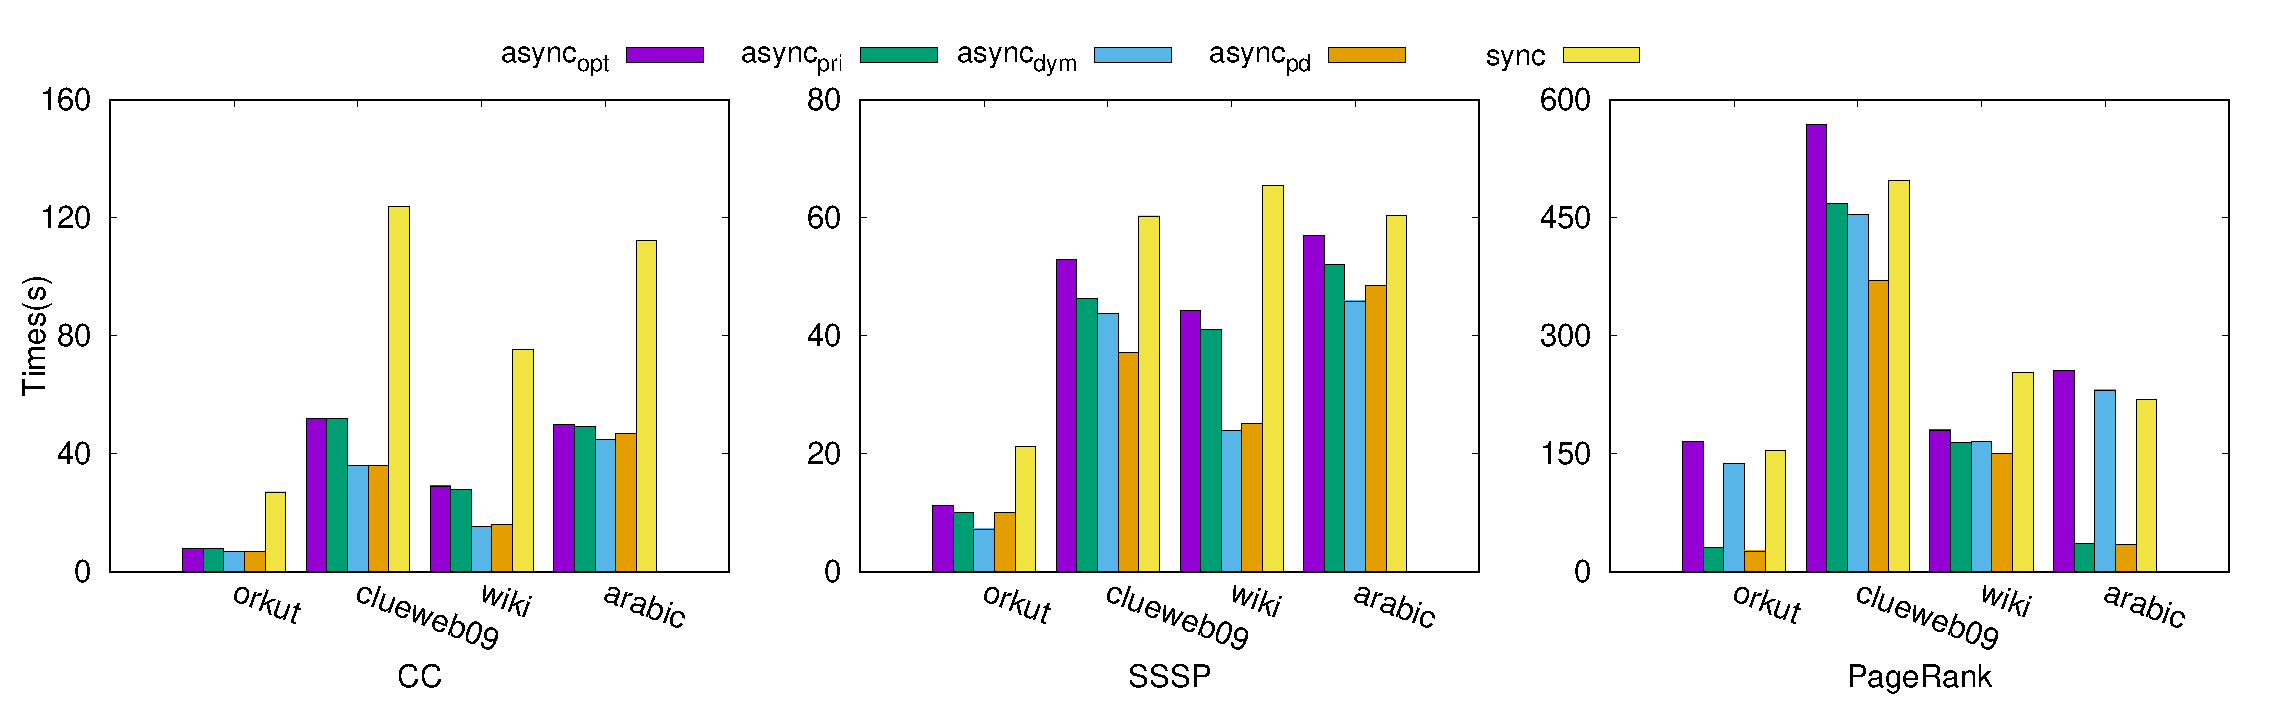
\includegraphics[width=6.6in]{figuration/summary.eps}
	\vspace{-0.1in}
	\caption{Effectiveness of Adaptive Message Buffer}
	\label{fig:summary}
	\vspace{-0.1in}
\end{figure*}
We perform the three algorithm with four dataset, we compare each query with five cases. Synchronous processing, Asynchronous processing, Asynchronous processing with fixed buffer using priority scheduling, Asynchronous processing with Adaptive sending buffer strategy. And Block-centric processing. To get the manual optimized buffer size, we fixed the buffersize to 500, 1000 and 2000 in turn, and choose the best one as result.  and the overall result is shown in figure \ref{fig:summary}.
For CC and SSSP algorithm, the Adaptive Message buffer strategy shows significent speed up over fixed buffer setting on clueweb09 ahd wiki, says1.7 to   

\begin{comment}
\begin{table*}[!t]
	%\vspace{-0.1in}
	\caption{Performance when varying workloads ($d$ is diameter, $e$ is powerlaw exponent)}
	\vspace{-0.0in}
	\hspace{-0.3in}
	\label{tab:wrokload}
	%\centering
	\scriptsize
	\begin{tabular}{c|c|c|c|c|c|c|c|c|c|c|c}
		\hline
		\multirow{2}{*}{\textbf{Dataset}} & \multirow{2}{*}{\tabincell{c}{\textbf{Nodes}}} & \multirow{2}{*}{\tabincell{c}{\textbf{Edges}}} & \multirow{2}{*}{\tabincell{c}{\textbf{Graph}\\ \textbf{type}}} & \multirow{2}{*}{\tabincell{c}{\textbf{$d$}}}& \multirow{2}{*}{\tabincell{c}{\textbf{$e$}}} & \multicolumn{3}{|c}{\textbf{SSSP}} & \multicolumn{3}{|c}{\textbf{PageRank}} \\
		\cline{7-12}
		&  & & & & & \textbf{Sync.} & \textbf{Async.} & \footnotesize{\textbf{Speedup}} & \textbf{Sync.} & \textbf{Async.} & \footnotesize{\textbf{Speedup}}\\
		\hline\hline
		\textbf{Actor} & 382,219 & 33,115,812 & collaborate & 13 & 2.131 & 34.62s & 1.54s & 22.44X & 63.62s & 7.03s & 9.05X \\
		\hline
		\textbf{Amazon} & 403,394 & 3,387,388 & co-purchase & 25 & 3.151 & 79.18s & 1.55s & 51.05X & 53.77s & 1.02s & 52.9X \\
		\hline
		\textbf{arXiv} & 28,093 & 4,596,803 & co-author & 9 & 1.731 & 19.7s & 1.51s & 13.03X & 53.2s & 1.01s & 52.7X \\
		\hline
		\textbf{DBLP} & 1,314,050 & 18,986,618 & co-author & 24 & 3.221 & 55.38s & 3.18s & 17.41X & 89.76s & 5.06s & 17.75X \\
		\hline
		\textbf{Flicker} & 2,302,925 & 33,140,017 & social & 23 & 1.711 & 38.3s & 3.95s & 9.71X & 84.24s & 24.2s & 3.48X \\
		\hline
		\textbf{Livejournal} & 5,204,176 & 49,174,464 & social & 23 & 1.537 & 57.26s & 9.41s & 6.08X & 111.09s & 49.43s & \textcolor{blue}{\textbf{2.25X}} \\
		\hline
		\textbf{Orkut} & 3,072,441 & 117,184,899 & social & 10 & 1.272 & 58.99s & 14.07s & \textcolor{blue}{\textbf{4.19X}} & 187.74s & 16.18s & 11.6X \\
		\hline
		\textbf{Patent-US} & 3,774,768 & 16,518,947 & citation & 26 & 4.001 & 66.83s & 3.21s & 20.8X & 68.06s & 6.11s & 11.15X \\
		\hline
		\textbf{Prosper} & 89,269 & 3,394,979 & loan & 8 & 2.191 & 37.75s & 1.51s & 24.93X & 52.61s & 1.02s & 51.58X \\
		\hline
		\textbf{RoadCA} & 1,965,206 & 2,766,607 & road net & 865 & 8.991 & 140.43s & 1.55s & 90.31X & 57.06s & 1.03s & \textcolor{red}{\textbf{55.59X}} \\
		\hline
		\textbf{RoadTX} & 1,379,917 & 1,921,660 & road net & 1064 & 8.901 & 137.2s & 1.55s & 88.4X & 54.49s & 1.02s & 53.63X \\
		\hline
		\textbf{Skitter} & 1,696,415 & 11,095,298 & Internet & 31 & 2.291 & 31.09s & 1.55s & 20.01X & 59.51s & 3.04s & 19.56X \\
		\hline
		\textbf{soc-LiveJ} & 4,847,571 & 68,475,391 & social & 20 & 2.651 & 67.2s & 11.2s & 6X & 113.51s & 39.2s & 2.9X \\
		\hline
		\textbf{soc-Pokec} & 1,632,803 & 30,622,564 & social & 14 & 3.081 & 53.85s & 4.81s & 11.19X & 76.83s & 15.1s & 5.09X \\
		\hline
		\textbf{TREC} & 1,601,787 & 8,063,026 & web & 112 & 2.231 & 130.84s & 1.6s & 81.62X & 55.29s & 2.03s & 27.23X \\
		\hline
		\textbf{\footnotesize{web-BerkStan}} & 685,230 & 7,600,595 & web & 208 & 2.601 & 692.08s & 3.1s & \textcolor{red}{\textbf{222.82X}} & 54.13s & 2.02s & 26.76X \\
		\hline
		\textbf{web-Google} & 875,713 & 5,105,039 & web & 24 & 2.731 & 70.8s & 1.59s & 44.64X & 54.24s & 2.03s & 26.67X \\
		\hline
		\textbf{Wiki-Talk} & 2,987,535 & 24,981,163 & communicate & 9 & 1.811 & 23.81s & 3.1s & 7.68X & 83.57s & 28.27s & 2.96X \\
		\hline
		\textbf{Youtube-u} & 3,223,589  & 9,375,374 & social & 31 & 2.211 & 30.6s & 2.43s & 12.6X & 65.91s & 5.08s & 12.96X \\
		\hline
		\textbf{\footnotesize{Zhishi-Baidu}} & 2,141,300 & 17,794,839 & web & 20 & 2.291 & 49.19s & 3.29s & 14.96X & 66.72s & 8.09s & 8.25X\\
		\hline
	\end{tabular}
	\vspace{-0.1in}
\end{table*}
\end{comment}

\Paragraph{Convergence and buffer changes}
\begin{figure*}[!t]
	\vspace{0.0in}
	\centering
	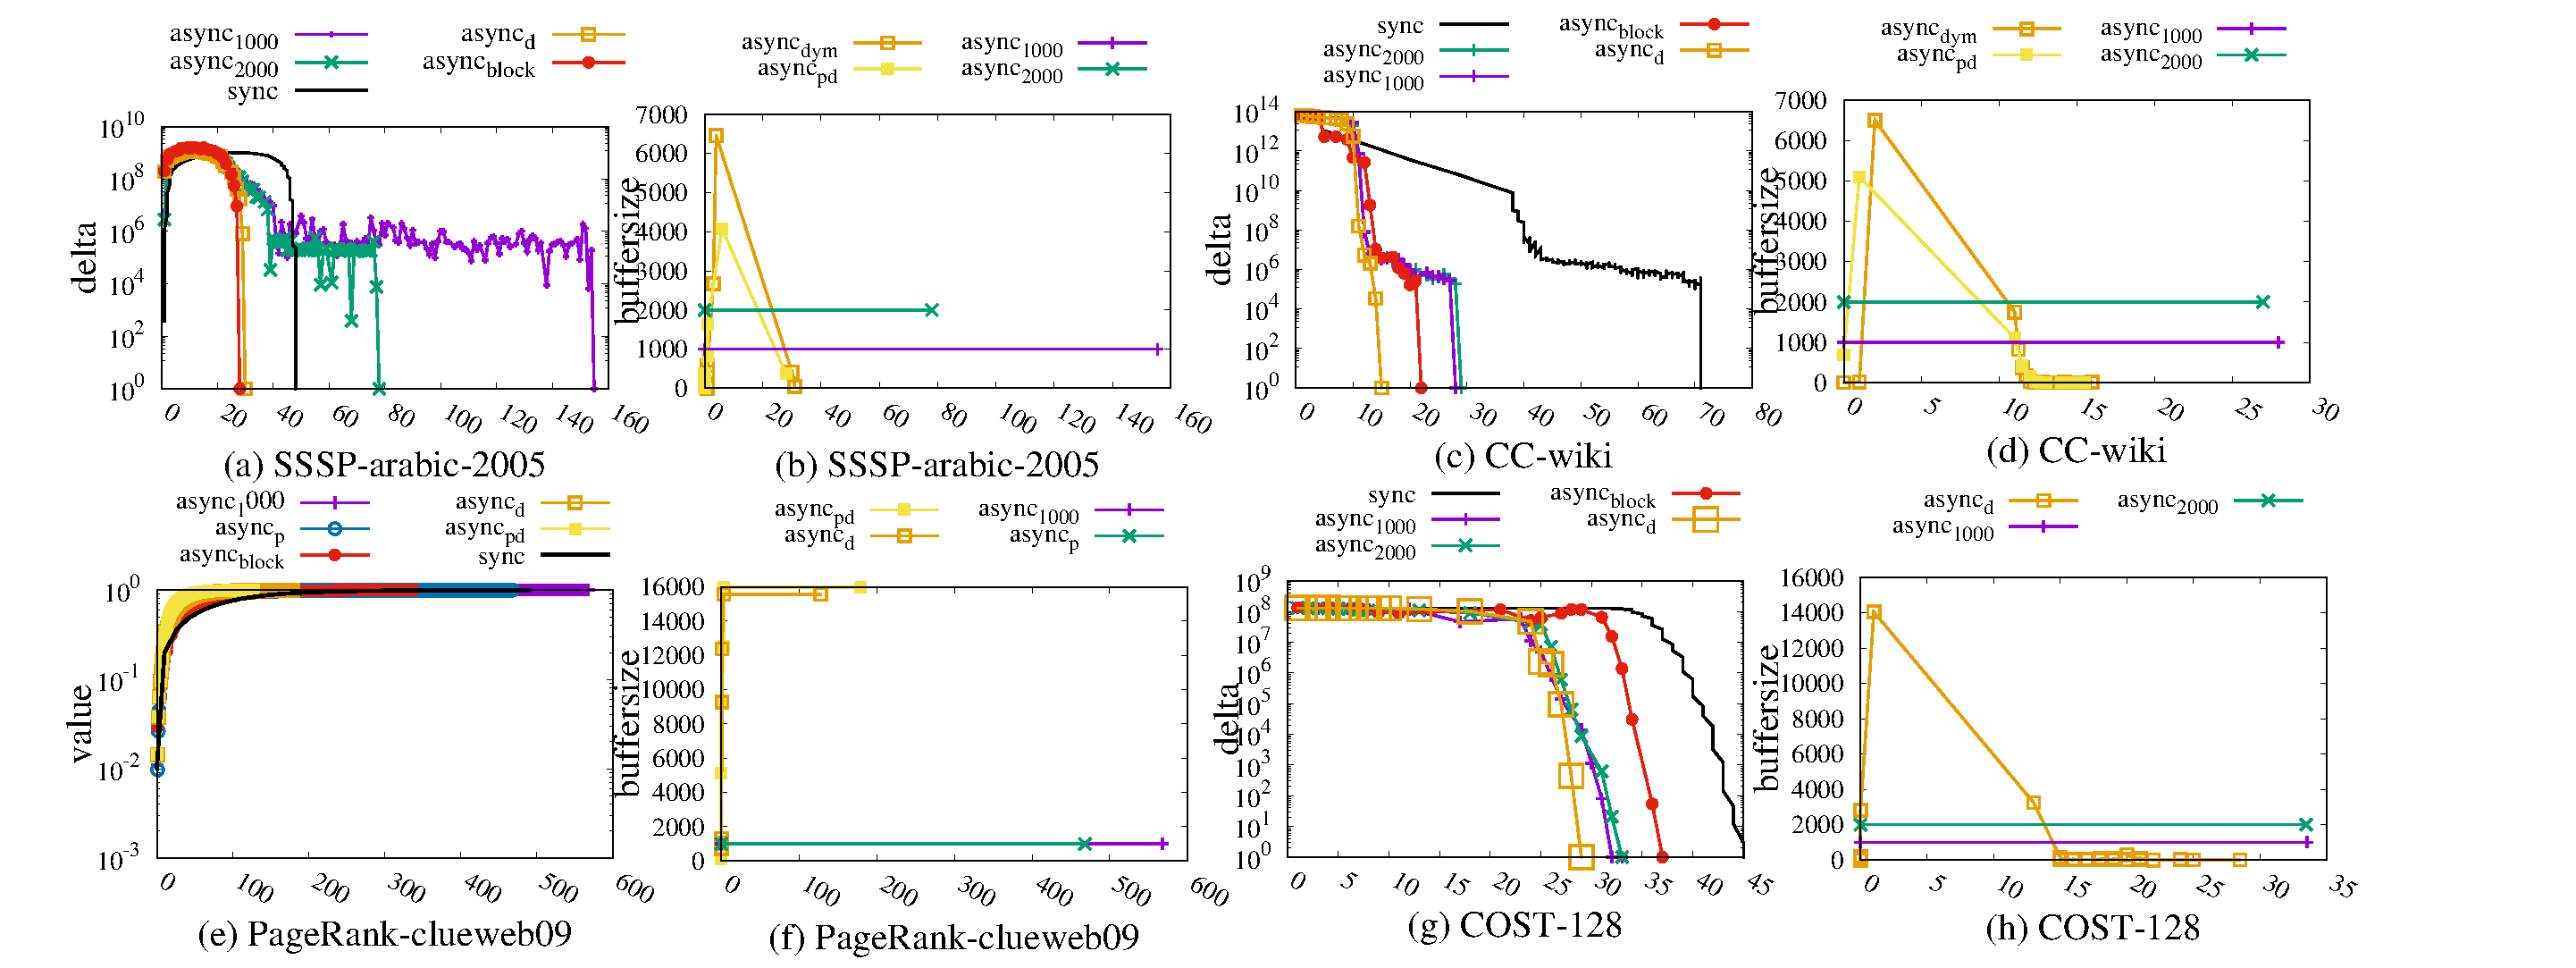
\includegraphics[width=6.6in]{figuration/combine.eps}
	\vspace{-0.1in}
	\caption{Effectiveness of Adaptive Message Buffer}
	\label{fig:details}
	\vspace{-0.1in}
\end{figure*}
%In order to analyze the factors for performance improvement and eliminate the interference from system implementation factors, we also implement a synchronous version of A3Log, which uses synchronous semi-naive evaluation (i.e., synchronous accumulated recursive programs). In addition, we turn off the scheduling then it shows the performance ahieved by pure asynchronous aggregation.

%\noindent\textbf{Algorithms and Datasets}
%We test more algorithms to see the effect variations on different workloads, including Least Common Ancestor(LCA), ``What is the cost of each part?'' (COST), ``Who will come to the party?'' (PARTY), and ``Computing Paths in a DAG'' (PATH). More details of these algorithms can be found in \cite{fullversion}. For LCA, we use a citation network Patent-US \cite{konect}. For COST, we synthetically generate a hierarchical (tree-like) dataset with 64000000 tree nodes. PARTY is a graph based algorithm, so we use the same ClueWeb20M dataset. For PATH, we synthetically generate a directed acyclic graph (DAG) dataset with 4915 nodes and 56148 edges. PATH is a computation intensive workload since it evaluates the paths between all pairs.


%We run these algorithms on the an r3.8xlarge EC2 instance with 32 vCPUs and 244GB memory. All these experiments are run with 32 threads. Fig. \ref{fig:single-optimize} shows the results. The runtime by synchronous semi-naive evaluation is considered as the baseline. The speedups from asynchronous execution and prioritized scheduling exhibit variations for different workloads. Generally speaking, the graph based algorithms benefit from asynchronous aggregation and priority scheduling more. For SSSP and PageRank, great performance gains are achieved by priority scheduling. However, for COST, the priority scheduling brings negative effect. This is because that COST aims to compute all parts' cost in a hierarchical structure and the computations on these parts equally contribute to the output. Using priority scheduling will not bring any benefit but only incurs scheduling overhead. However, we still take advantage of asynchronous aggregation to achieve better performance.


 \subsection{Scaling Performance}
 \label{sec:expr:scale}
 \begin{comment}

 \begin{figure}[!t]
 	\centering
 	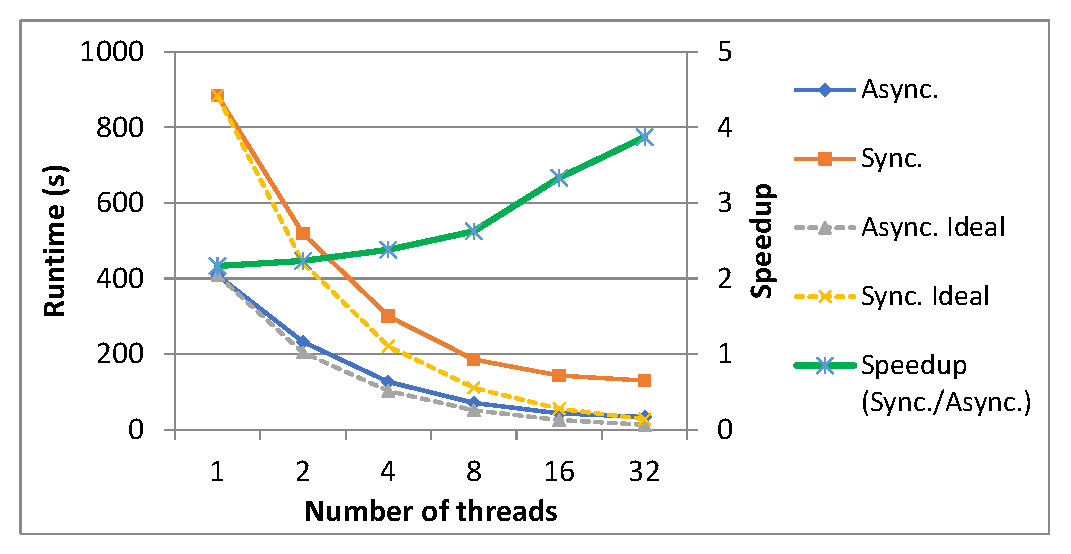
\includegraphics[width=2.8in]{fig/single-scalability}
 	\vspace{-0.1in}
 	\caption{Scaling performance (many-core)}
 	\label{fig:single-scalability}
 \end{figure}

 \begin{figure}[!t]
 	\centering
 	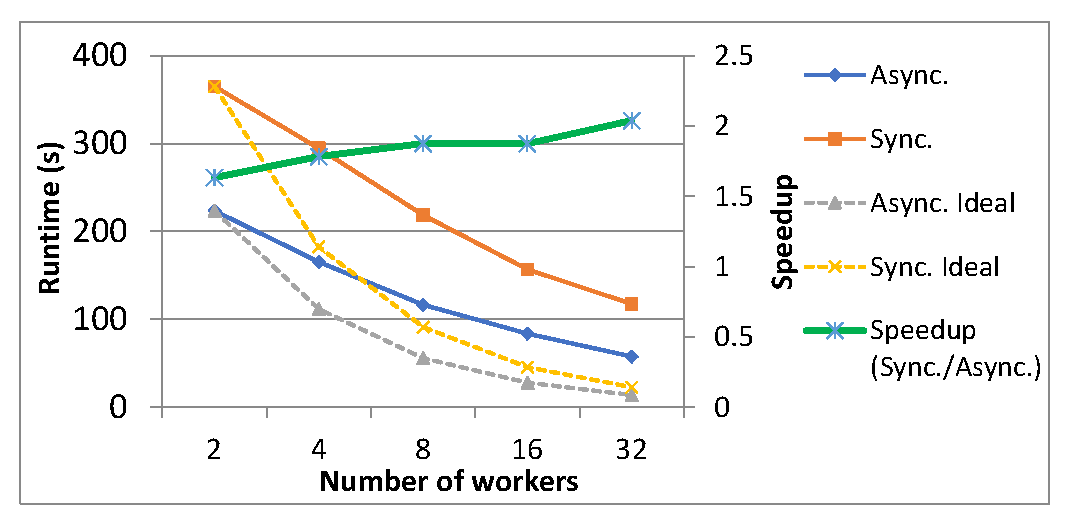
\includegraphics[width=2.8in]{fig/dist-scalability}
 	\vspace{-0.1in}
 	\caption{Scaling performance (distributed)}
 	\label{fig:dist-scalability}
 \end{figure}
\end{comment}
\begin{figure}[!t]
	\vspace{0.0in}
	\centering
	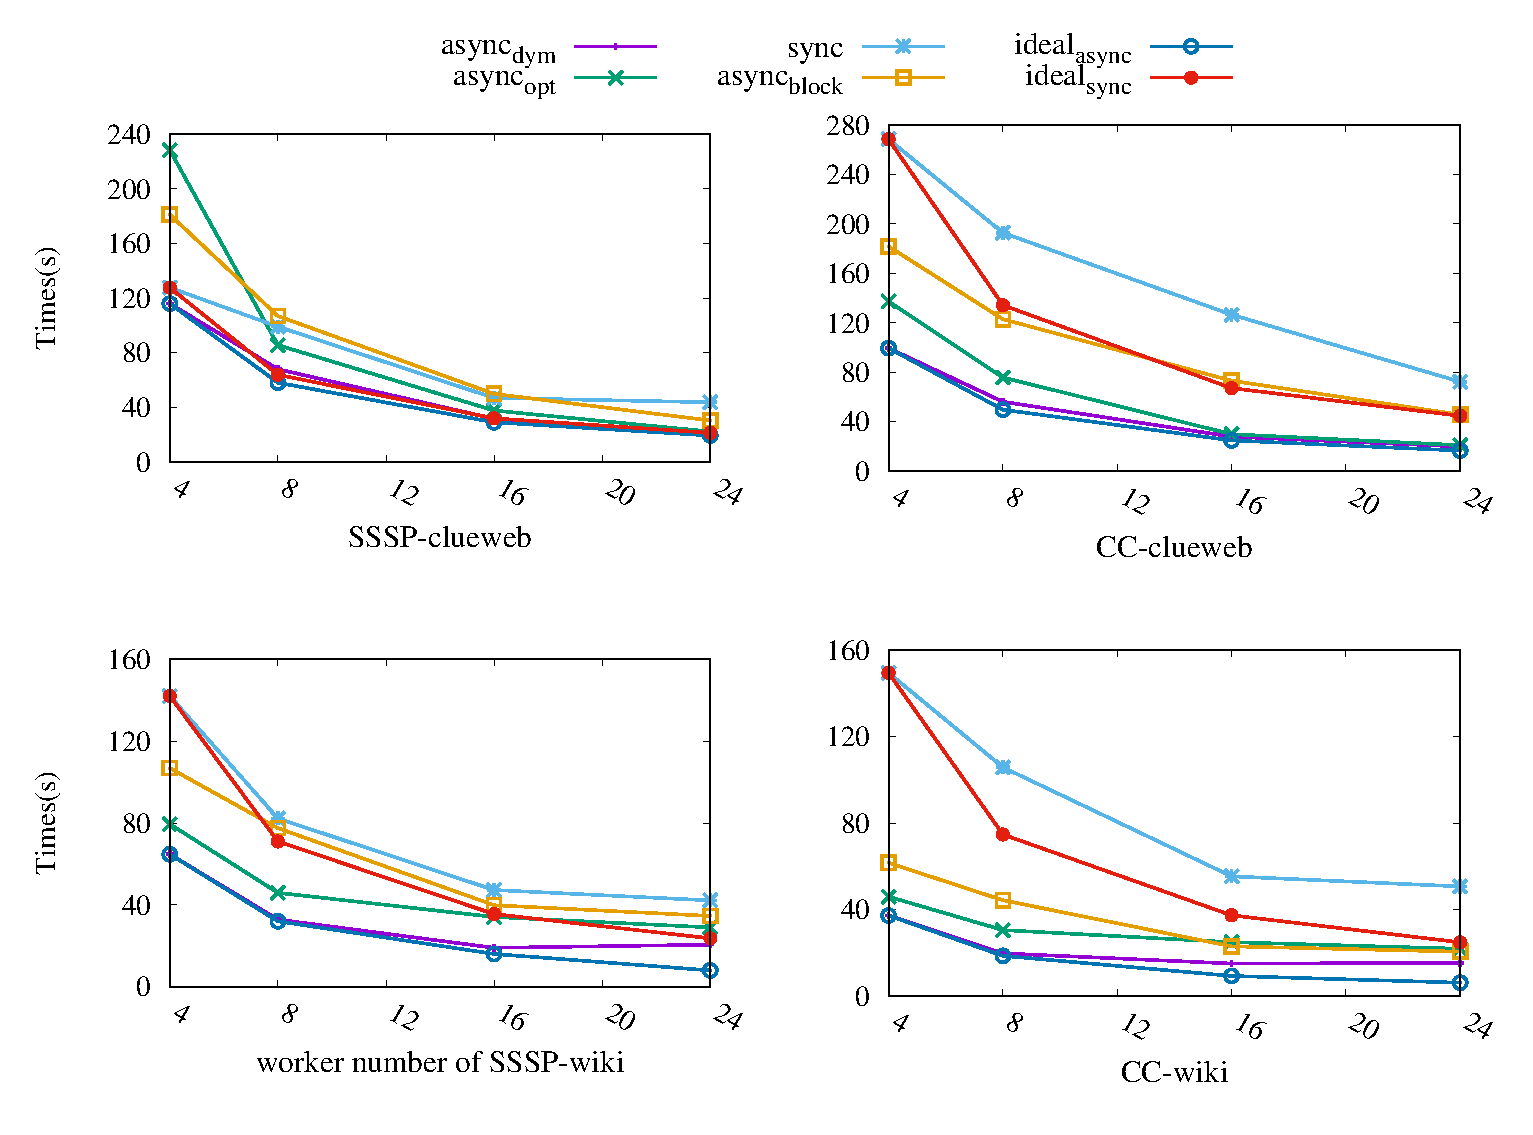
\includegraphics[width=3.4in]{figuration/scale.eps}
	\vspace{-0.1in}
	\caption{ScalePerformance}
	\label{fig:scale}
	\vspace{-0.1in}
\end{figure}
%asynchronous aggregation is expected to achieve better scaling performance. We evaluate the scaling performance of A3Log's share-memory runtime on an r3.8xlarge EC2 instance. We perform PageRank computation with the synchronous and asynchronous versions (without scheduling) of A3Log and vary the number of threads from 1 to 32. The runtime results are shown in Fig.\ref{fig:single-scalability}. We also draw the ideal scaling performance curve based on the runtime result of 1 thread. The asynchronous A3Log's scaling performance curve is closer to its ideal curve, while the synchronous A3Log exhibits larger difference to its ideal curve when running on more threads. Asynchronous execution also shows higher speedup over synchronous execution when running on more threads.

% We also evaluate the scaling performance of A3Log's distributed runtime on a cluster with a number of c4.large EC2 instances, each with 2 vCPUs and 3.75GB memory. We perform PageRank computation with the synchronous and asynchronous executions (without scheduling) and vary the number of workers from 1 to 32. The runtime results are shown in Fig. \ref{fig:dist-scalability}. We also draw the ideal scaling performance curve based on the runtime result of 2-workers. Similar to the results on shared-memory runtime, asynchronous execution also shows better scaling performance. Higher speedup over synchronous execution is achieved when running on larger size cluster.


%\subsection{Comparison with Different Workloads}
%\label{sec:expr:workloads}
%To see the performance when varying datasets, we choose 20 various graph datasets with various graph structures and various graph properties. All the datasets are downloaded from \cite{konect}. We use two typical graph algorithms SSSP and PageRank for evaluation. We run the shared-memory version of A3Log on a c4-2xlarge EC2 instance with 8 vCPU and 60GB memory. A3Log is configured with 8 threads. We compare the algorithm runtime of synchronous execution and asynchronous execution on these graphs.

%Table \ref{tab:wrokload} shows the graph datasets and the runtime results. The asynchronous execution exhibits 4.19X-222.82X speedup over synchronous execution on SSSP computation, and 2.25X-55.59X speedup over synchronous execution on PageRank computation. Generally speaking, asynchronous SSSP achieves higher speedup on large diameter graphs, and asynchronous PageRank computation achieves higher speedup on the graphs with larger powerlaw exponent. Of course, the performance speedup also relates to the graph structures and graph types. %Note that, in asynchronous execution, the termination check is performed periodically (every 1 second in this experiment). If the runtime results of asynchronous executions shows 1.x second, they may converge less than 1 second. Thus, the performance of asynchronous execution is expected to be even higher.

 %\subsection{Effectiveness of Aggregate Operations}
 %\label{sec:expr:aggregations}
 \begin{comment}
 \begin{figure}[!t]
 	\vspace{-0.1in}
 	\centerline{
 		\subfloat[RoadCA]{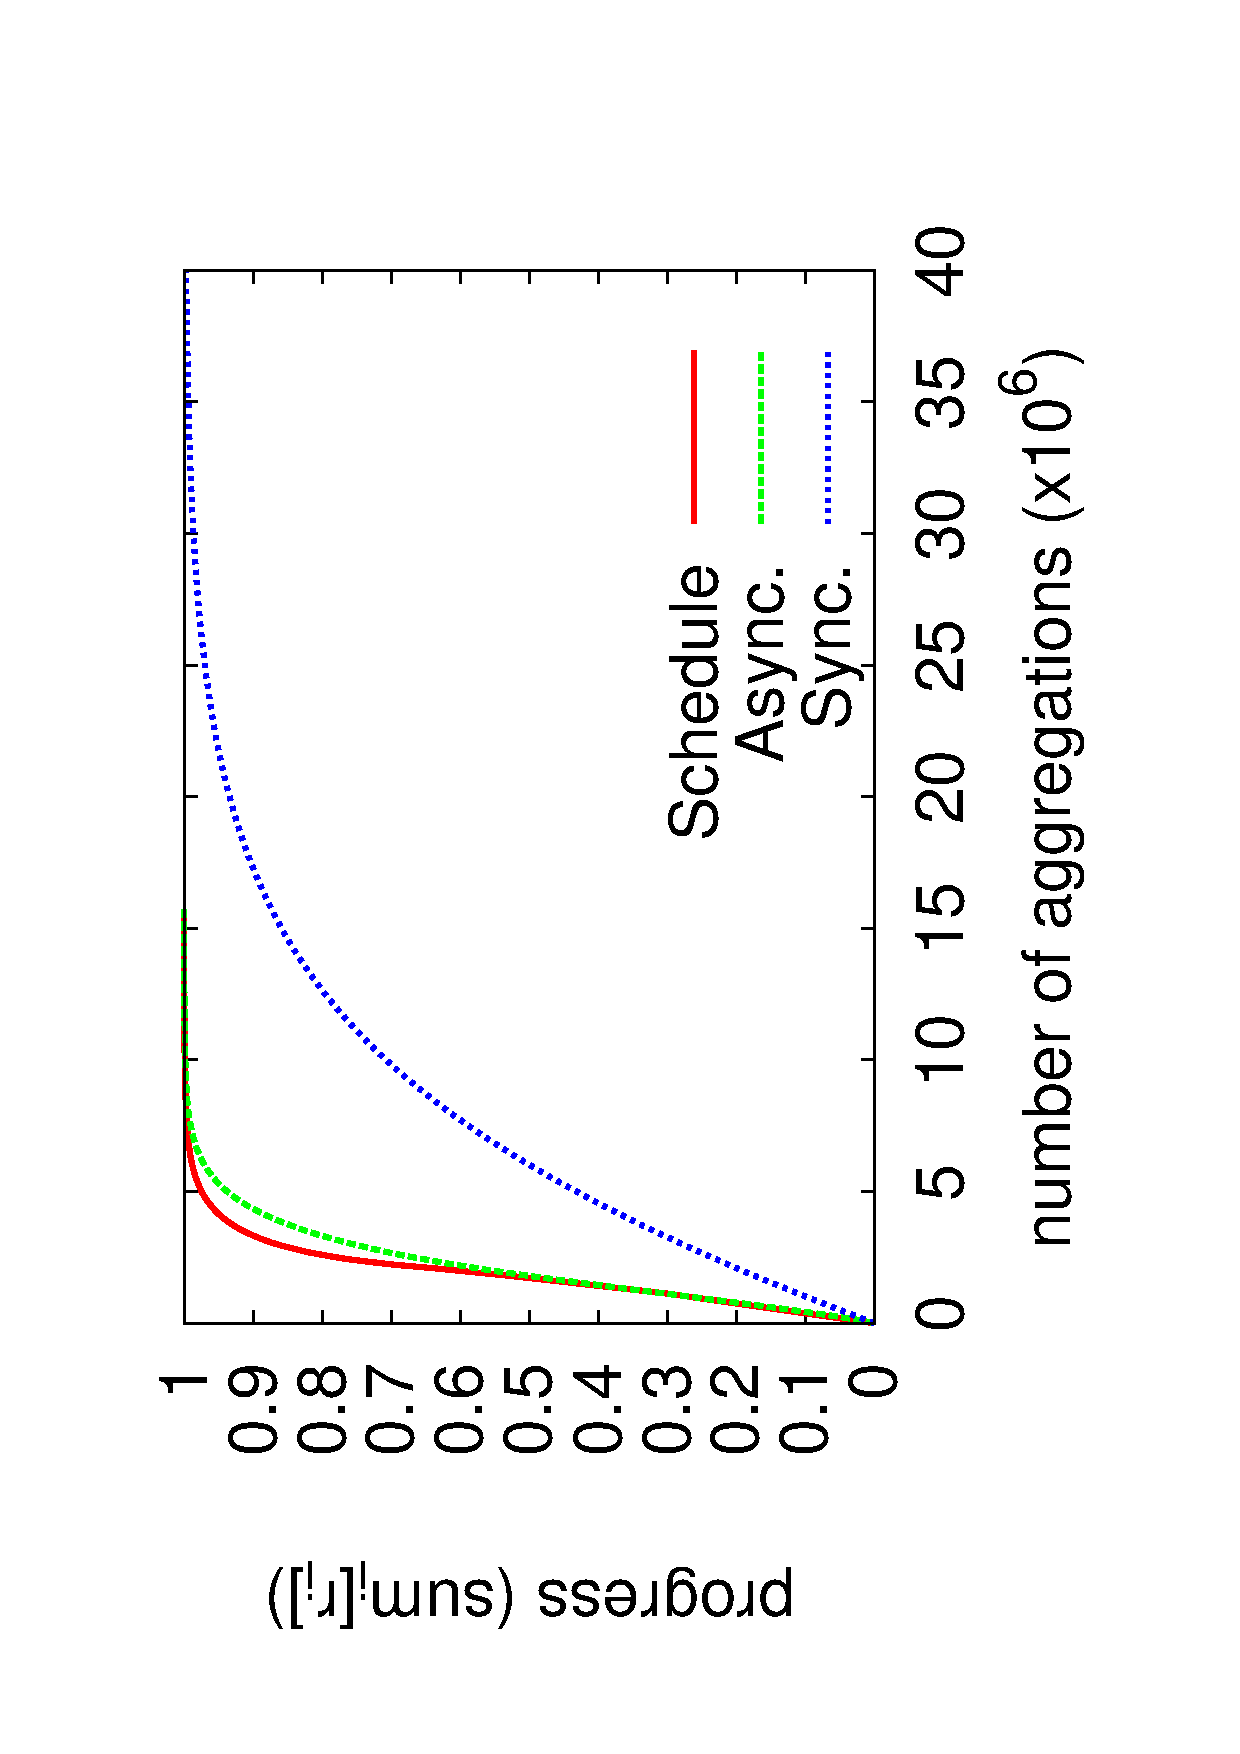
\includegraphics[width=1.3in, angle=-90]{fig/roadca_aggregate_progress}
 			\label{fig:single-numagg:roadca}
 			\vspace{-0.05in}}
 		\hspace{-5mm}
 		\subfloat[Livejournal]{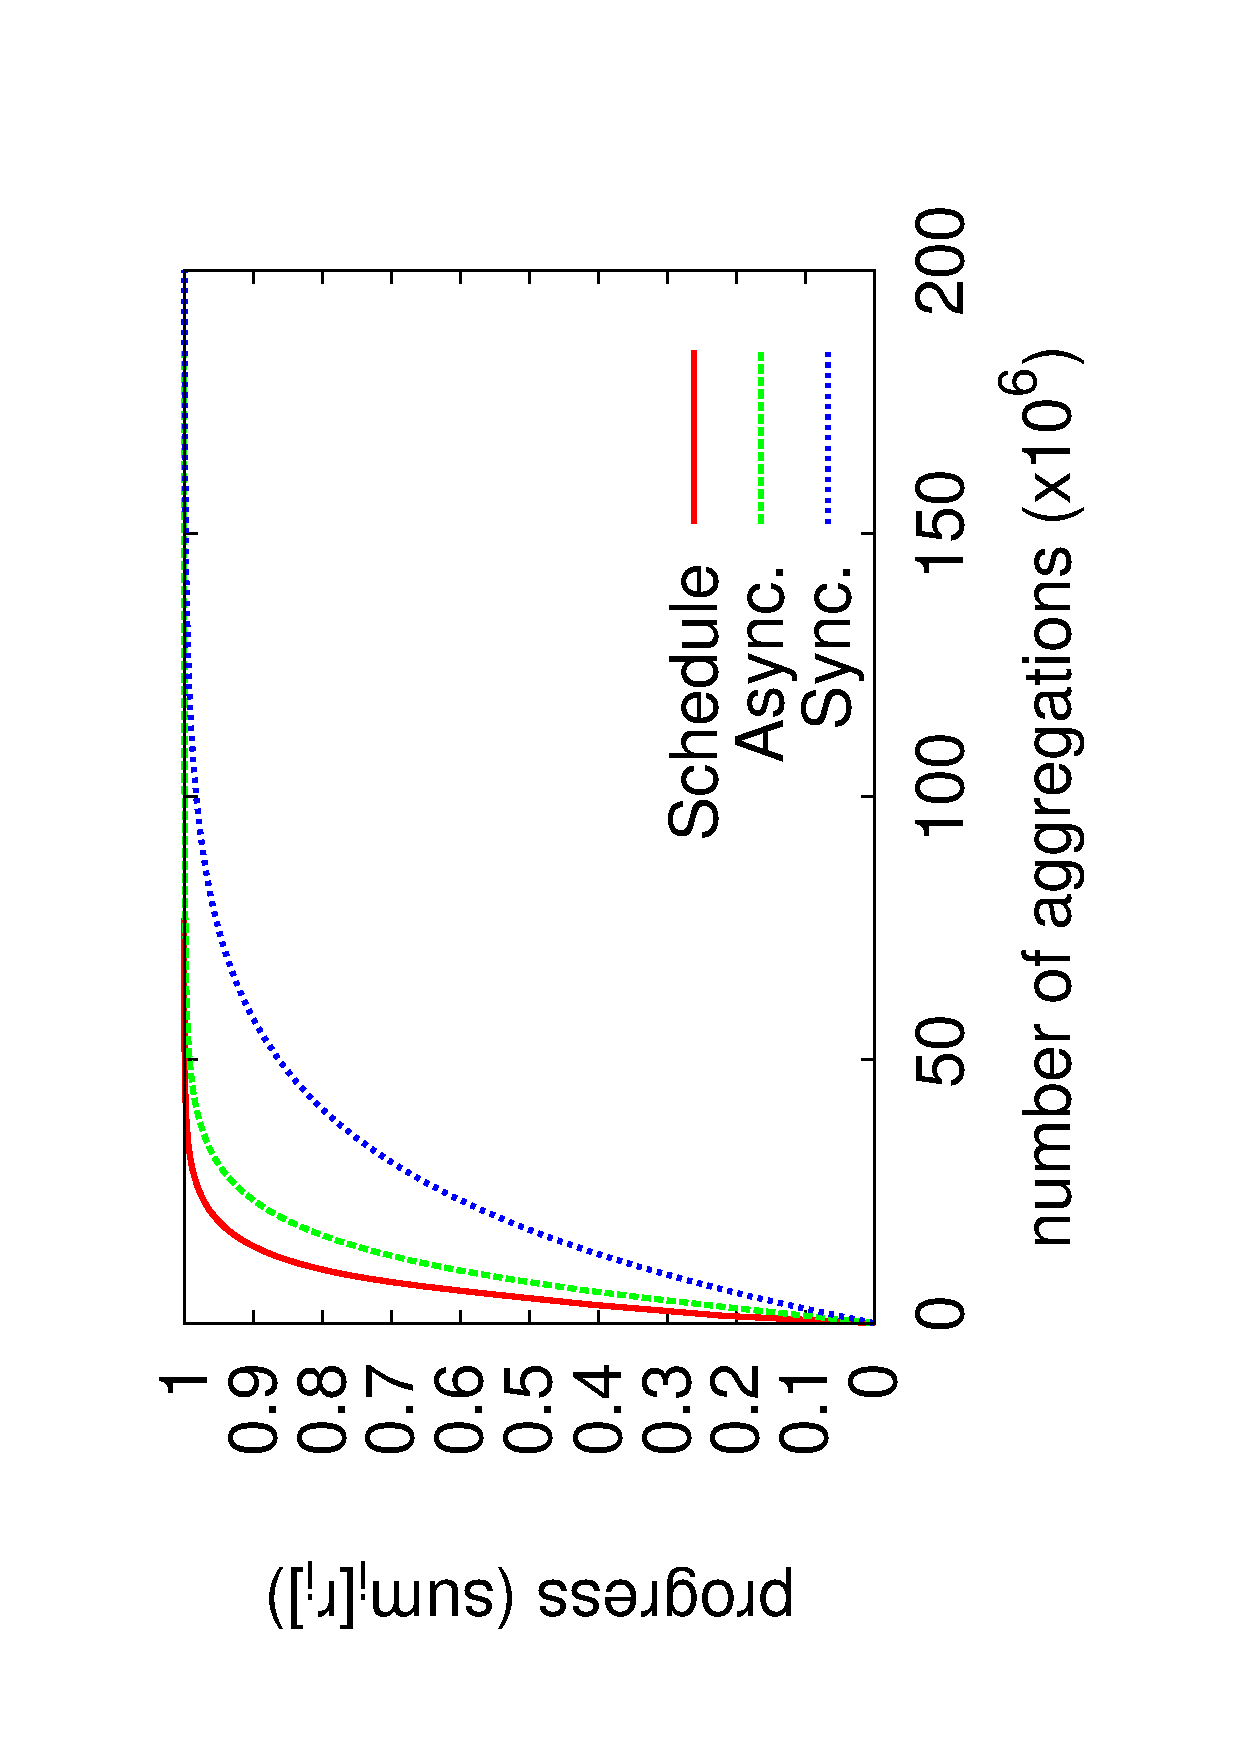
\includegraphics[width=1.3in, angle=-90]{fig/livejournal_aggregate_progress}
 			\label{fig:single-numagg:livejournal}
 			\vspace{-0.05in}}
 	}
 	\vspace{-0.1in}
 	\caption{Effectiveness of aggregate operations to converging progress}
 	\label{fig:single-numagg}
 	\vspace{-0.1in}
 \end{figure}
\end{comment}
 %In this experiment, we evaluate the effectiveness of asynchronous aggregations on accelerating the computation prog-ress.

 %We run PageRank on two datasets, RoadCA and Livejournal, which result in the most speedup and the least speedup comparing to synchronous aggregation as shown in Table \ref{tab:wrokload}. We record the accumulated number of aggregate operations during the computation. In the accumulated version of PageRank (see Sec. \ref{sec:async:convert}), the summation of ranking scores $\sum_i{r_i}$ is approaching to 1 and will finally converge to 1. So we estimate the computation progress by evaluating $\sum_i{r_i}$ periodically. Fig. \ref{fig:single-numagg} shows the results. By using asynchronous aggregation, the converging progress is much faster than using synchronous execution. The scheduling of aggregate operations will further speedup the progress. The asynchronous aggregation with scheduling shows more effectiveness, so that each aggregate operation contributes more. It also shows more effectiveness on the RoadCA graph than on the Lievejournal graph. This is the reason why higher speedup is observed on the RoadCA graph.

\section{Related Works}
\label{sec:related}

%\noindent\textbf{Coordination Avoidance} Minimizing coordination, or blocking communication between concurrently executing operations, is key to maximizing scalability, availability, and high performance in database systems. However, uninhibited coordination-free execution can compromise application correctness, or consistency. Coordination and consistency are the most critical issues for system performance and manageability at scale \cite{Bailis:2014:CAD:2735508.2735509}. Hellerstein et al. have set up the foundation \cite{Hellerstein:2010:DIE:1860702.1860704} and have put a lot of efforts to advance this field \cite{Alvaro:2013:CWB:2523616.2523632,Bailis:2014:QEC:2632661.2632792}. Dedalus \cite{Alvaro:2010:DDT:2185923.2185942} is proposed as a declarative foundation for the two signature features of distributed systems: mutable state, and asynchronous processing and communication. CALM (Consistent and Logical Monotonicity) principle \cite{calm} is described for reasoning about distributed system behaviour, which ensures eventual consistency by enforcing a \emph{monotonic} logic. A declarative language called Bloom \cite{Conway:2012:LLD:2391229.2391230} that encourages CALM programming and is well-suited to the inherent characteristics of distribution. Edelweiss \cite{Conway:2014:EAS:2732279.2732285} is a sublanguage of Bloom that provides an Event Log Exchange (ELE) programming model, yet automatically reclaims space without programmer assistance, which can be used to elegantly implement asynchronous communications. Blaze \cite{blaze} ensures consistent outcomes via a more efficient and manageable protocol of asynchronous point-to-point communication between producers and consumers. MacroBase \cite{Bailis:2017:MPA:3035918.3035928} is a fast data system built to explore the fast data principles that suggests asynchronously prioritizing computation on inputs that most affect outputs.



\noindent\textbf{Asynchronous Computation in Graph Analytics} Asynchronous computation has attracted much attention in the field of graph processing. GraphLab \cite{Low:2012:DGF:2212351.2212354} aims to express asynchronous iterative algorithms with sparse computational dependencies while ensuring data consistency and achieving good parallel performance. Frog \cite{8017445} is a lock-free semi-asynchronous parallel graph processing framework with a graph coloring model. Grace \cite{grace} is a single-machine parallel graph processing platform that allows customization of vertex scheduling and message selection to support asynchronous computation. Giraph++ \cite{Tian:2013:TLV:2732232.2732238} not only allows asynchronous computation while keeping the vertex-centric model but also is able to handle mutation of graphs. GiraphUC \cite{Han:2015:GUB:2777598.2777604} relies on barrierless asynchronous parallel (BAP), which reduces both message staleness and global synchronization. Maiter \cite{maiter} proposes delta-based asynchronous iterative computation model (DAIC) and supports distributed asynchronous graph processing. GunRock \cite{Wang:2016:GHG:2851141.2851145} supports fast asynchronous graph computation in GPUs. Unfortunately, the above graph systems do not support automatic asynchronization.

%Asynchronous MapReduce \cite{asynchronous} proposes to use more local synchronizations to replace global synchronizations to gain performance.

GRAPE \cite{Fan:2017:PSG:3035918.3035942} differs from prior systems in its ability to automatically parallelize existing sequential graph algorithms as a whole. Sequential graph algorithms can be "plugged into" GRAPE with minor changes, and get parallelized. As long as the sequential algorithms are correct, the GRAPE parallelization guarantees to terminate with correct answers under a monotonic condition. However, GRAPE cannot automatically asynchronize a sequential graph algorithm.

%compare with Maiter \cite{maiter}, extended to relational algebral, generalize to aggregation, support to automatically asyncronization, datalog system.
\begin{comment}
\noindent\textbf{Asynchronous Computation in Machine Learning} In machine learning, some algorithms with non-serializable lock-free implementations offer significant speedups. Gonzalez et al. \cite{DBLP:journals/corr/GonzalezBJFHGS15} examine the growing gap between efficient machine learning algorithms exploiting asynchrony and fine-grained communication, and commodity distributed dataflow systems (Hadoop and Spark) that are optimized for coarse-grained models. Google DeepMind group recently proposes asynchronous methods for deep reinforcement learning \cite{Mnih:2016:AMD:3045390.3045594}, which surpasses the current state-of-the-art on the Atari domain while training for half the time on a single multi-core CPU instead of a GPU. DimmWitted \cite{Zhang:2014:DSM:2732977.2733001} exposes a range of options for asynchronous data sharing, which outperforms general cluster compute frameworks by orders of magnitude in the context of popular models, including SVMs, logistic regression, Gibbs sampling, and neural networks. HOGWILD! \cite{Niu:2011:HLA:2986459.2986537} is a implementation of stochastic gradient descent (SGD), which places a single copy of the model in the memory of a multi-core server and runs multiple worker processes that simultaneously run gradient steps in parallel. An asynchronous parallel stochastic coordinate descent algorithm is proposed in \cite{Liu:2015:APS:2789272.2789282}, which shows significant speedup in multi-core environment. A burgeoning cottage industry of machine learning researchers has begun to extend asynchronous execution strategies to an increasing number of optimization tasks.
\end{comment}
\noindent\textbf{Datalog Systems}
Besides SociaLite \cite{Lam:2013:SDE:2510649.2511289,Seo:2013:DSD:2556549.2556572} and Myria \cite{Halperin:2014:DMB:2588555.2594530,Wang:2015:AFR:2824032.2824052}, there exist other Datalog systems. DeALS \cite{Shkapsky:2013:GQN:2536274.2536290,7113340} is a deductive database systems relying on Datalog language, supporting optimized execution over diverse platforms including sequential implementations, multi-core machines, and clusters. BigDatalog \cite{Shkapsky:2016:BDA:2882903.2915229} is built on top of Spark \cite{Zaharia:2010:SCC:1863103.1863113} and provides declarative semantics of monotonic aggregate programs. Datalography \cite{7840589} incorporates optimization techniques for efficient distributed evaluation of Datalog queries on Giraph \cite{giraph}. LogicBlox \cite{Aref:2015:DIL:2723372.2742796} is a commercial database system based on LogiQL.

\section{Conclusions}
\label{sec:conclusion}
We have presented A3, Automatic Asynchronous Aggregation. We clearly define the correctness conditions for asynchronous recursive aggregation and propose a technique to allow automatic asynchronization. We design and implement a Datalog system, A3Log, to support automatic asynchronous computation of the user's program and further proposed Dynamic message buffer strategy to optimize asynchonous performance. Our results show that A3Log shows better performance against the state-of-the-art Datalog systems for various applications. And optimized asynchronous processing shows better performance than the  synchronous version
%{\color{red}Here I wanna add something about Partition sensitive}


%\section{Related Works}
\label{sec:related}

%\noindent\textbf{Coordination Avoidance} Minimizing coordination, or blocking communication between concurrently executing operations, is key to maximizing scalability, availability, and high performance in database systems. However, uninhibited coordination-free execution can compromise application correctness, or consistency. Coordination and consistency are the most critical issues for system performance and manageability at scale \cite{Bailis:2014:CAD:2735508.2735509}. Hellerstein et al. have set up the foundation \cite{Hellerstein:2010:DIE:1860702.1860704} and have put a lot of efforts to advance this field \cite{Alvaro:2013:CWB:2523616.2523632,Bailis:2014:QEC:2632661.2632792}. Dedalus \cite{Alvaro:2010:DDT:2185923.2185942} is proposed as a declarative foundation for the two signature features of distributed systems: mutable state, and asynchronous processing and communication. CALM (Consistent and Logical Monotonicity) principle \cite{calm} is described for reasoning about distributed system behaviour, which ensures eventual consistency by enforcing a \emph{monotonic} logic. A declarative language called Bloom \cite{Conway:2012:LLD:2391229.2391230} that encourages CALM programming and is well-suited to the inherent characteristics of distribution. Edelweiss \cite{Conway:2014:EAS:2732279.2732285} is a sublanguage of Bloom that provides an Event Log Exchange (ELE) programming model, yet automatically reclaims space without programmer assistance, which can be used to elegantly implement asynchronous communications. Blaze \cite{blaze} ensures consistent outcomes via a more efficient and manageable protocol of asynchronous point-to-point communication between producers and consumers. MacroBase \cite{Bailis:2017:MPA:3035918.3035928} is a fast data system built to explore the fast data principles that suggests asynchronously prioritizing computation on inputs that most affect outputs.



\noindent\textbf{Asynchronous Computation in Graph Analytics} Asynchronous computation has attracted much attention in the field of graph processing. GraphLab \cite{Low:2012:DGF:2212351.2212354} aims to express asynchronous iterative algorithms with sparse computational dependencies while ensuring data consistency and achieving good parallel performance. Frog \cite{8017445} is a lock-free semi-asynchronous parallel graph processing framework with a graph coloring model. Grace \cite{grace} is a single-machine parallel graph processing platform that allows customization of vertex scheduling and message selection to support asynchronous computation. Giraph++ \cite{Tian:2013:TLV:2732232.2732238} not only allows asynchronous computation while keeping the vertex-centric model but also is able to handle mutation of graphs. GiraphUC \cite{Han:2015:GUB:2777598.2777604} relies on barrierless asynchronous parallel (BAP), which reduces both message staleness and global synchronization. Maiter \cite{maiter} proposes delta-based asynchronous iterative computation model (DAIC) and supports distributed asynchronous graph processing. GunRock \cite{Wang:2016:GHG:2851141.2851145} supports fast asynchronous graph computation in GPUs. Unfortunately, the above graph systems do not support automatic asynchronization.

%Asynchronous MapReduce \cite{asynchronous} proposes to use more local synchronizations to replace global synchronizations to gain performance.

GRAPE \cite{Fan:2017:PSG:3035918.3035942} differs from prior systems in its ability to automatically parallelize existing sequential graph algorithms as a whole. Sequential graph algorithms can be "plugged into" GRAPE with minor changes, and get parallelized. As long as the sequential algorithms are correct, the GRAPE parallelization guarantees to terminate with correct answers under a monotonic condition. However, GRAPE cannot automatically asynchronize a sequential graph algorithm.

%compare with Maiter \cite{maiter}, extended to relational algebral, generalize to aggregation, support to automatically asyncronization, datalog system.

\noindent\textbf{Asynchronous Computation in Machine Learning} In machine learning, some algorithms with non-serializable lock-free implementations offer significant speedups. Gonzalez et al. \cite{DBLP:journals/corr/GonzalezBJFHGS15} examine the growing gap between efficient machine learning algorithms exploiting asynchrony and fine-grained communication, and commodity distributed dataflow systems (Hadoop and Spark) that are optimized for coarse-grained models. Google DeepMind group recently proposes asynchronous methods for deep reinforcement learning \cite{Mnih:2016:AMD:3045390.3045594}, which surpasses the current state-of-the-art on the Atari domain while training for half the time on a single multi-core CPU instead of a GPU. DimmWitted \cite{Zhang:2014:DSM:2732977.2733001} exposes a range of options for asynchronous data sharing, which outperforms general cluster compute frameworks by orders of magnitude in the context of popular models, including SVMs, logistic regression, Gibbs sampling, and neural networks. HOGWILD! \cite{Niu:2011:HLA:2986459.2986537} is a implementation of stochastic gradient descent (SGD), which places a single copy of the model in the memory of a multi-core server and runs multiple worker processes that simultaneously run gradient steps in parallel. An asynchronous parallel stochastic coordinate descent algorithm is proposed in \cite{Liu:2015:APS:2789272.2789282}, which shows significant speedup in multi-core environment. A burgeoning cottage industry of machine learning researchers has begun to extend asynchronous execution strategies to an increasing number of optimization tasks.

\noindent\textbf{Datalog Systems}
Besides SociaLite \cite{Lam:2013:SDE:2510649.2511289,Seo:2013:DSD:2556549.2556572} and Myria \cite{Halperin:2014:DMB:2588555.2594530,Wang:2015:AFR:2824032.2824052}, there exist other Datalog systems. DeALS \cite{Shkapsky:2013:GQN:2536274.2536290,7113340} is a deductive database systems relying on Datalog language, supporting optimized execution over diverse platforms including sequential implementations, multi-core machines, and clusters. BigDatalog \cite{Shkapsky:2016:BDA:2882903.2915229} is built on top of Spark \cite{Zaharia:2010:SCC:1863103.1863113} and provides declarative semantics of monotonic aggregate programs. Datalography \cite{7840589} incorporates optimization techniques for efficient distributed evaluation of Datalog queries on Giraph \cite{giraph}. LogicBlox \cite{Aref:2015:DIL:2723372.2742796} is a commercial database system based on LogiQL.

\section{Conclusions}
\label{sec:conclusion}

We have presented A3, Automatic Asynchronous Aggregation. We clearly define the correctness conditions for asynchronous recursive aggregation.  We also propose a technique to allow automatic asynchronization. We further design and implement a Datalog system, A3Log, to support automatic asynchronous computation of the user's program. A3Log provides both shared-memory runtime and distributed runtime. Our results show that A3Log shows comparable and most time better performance against the state-of-the-art systems for various applications.
{\color{red}Here I wanna add something about Partition sensitive}




% The following two commands are all you need in the
% initial runs of your .tex file to
% produce the bibliography for the citations in your paper.
\bibliographystyle{abbrv}
\bibliography{vldb_sample}  % vldb_sample.bib is the name of the Bibliography in this case
% You must have a proper ".bib" file
%  and remember to run:
% latex bibtex latex latex
% to resolve all references


%APPENDIX is optional.
% ****************** APPENDIX **************************************
% Example of an appendix; typically would start on a new page
%pagebreak--

\begin{appendix}
%You can use an appendix for optional proofs or details of your evaluation which are not absolutely necessary to the core understanding of your paper. 
\section{proofs}
\subsection{Proof of Theorem Monotonic}

\begin{proof}
	\label{sec:app:proof:monotonic}
	It is known that $\Delta Y^k=F(\Delta X^k)$and $\Delta X^0=X^0$.
	\begin{align}
	&G\Big(\Delta Y^0\cup (F\circ G)(\Delta Y^0)\cup\ldots\cup (F\circ G)^k(\Delta Y^0)\Big)\notag \\
	=&G\Big(G(\Delta Y^0)\cup (F\circ G)(\Delta Y^0)\cup \ldots \cup (F\circ G)^k( \Delta Y^0)\Big)\tag{2}\\
	=&G\Big(F\circ G(\Delta Y^0)\cup (F\circ G)^2(\Delta Y^0)\cup \ldots \cup (F\circ G)^k(\Delta Y^0)\Big) \tag{3}\\
	=& \ldots \notag \\
	=&G\Big((F\circ G)^k(\Delta Y^0)\Big)\tag{4}\\
	=&(G \circ F)^{k+1}(X^0).\notag
	\end{align}
	Line 3 is true because of the accumulative property. Due to the monotonic property line 4 is true .By repeat applying these two properties, we can reduce the original formula to line 5, the result of normal recursive aggregation. 
\end{proof}

\subsection{Proof of Theorem Asynchronous}
 \begin{proof}
 \label{sec:app:proof:correct}
 In this proof, We assumed that $X$ can be divided into two disjoint subset $X_0$ and $X_1$. we exchange the subset belongs to any two  recursion, and then prove that they have the same formula with the origin form. This is the basic form which can generalize all the other situations.
 \begin{align}
 &G(\Delta X^0\cup \ldots \cup F\circ G(\Delta X^{i}_0 \cup \Delta X^{j}_1)\cup\ F\circ G(\Delta X^{j}_0 \cup \notag\\ &\Delta X^{i}_1) \ldots\cup \Delta X^n)\tag{1} \\
 =&G( \ldots \cup G \circ F\circ G(\Delta X^{i}_0 \cup \Delta X^{{j}}_1)\cup\ G \circ F\circ G(\Delta X^{{j}}_0 \cup \notag\\ &\Delta X^{i}_1) \ldots)\tag{2} \\
 =&G( \ldots \cup G \circ F(\Delta X^{i}_0 \cup \Delta X^{{j}}_1)\cup\ G \circ F(\Delta X^{{j}}_0 \cup \Delta X^{{i}}_1) \ldots)\tag{3} \\
  =&G( \ldots \cup (G\circ F(\Delta X^{i}_0) \cup G\circ F(\Delta X^{{j}}_1))\cup\ (G \circ F(\Delta X^{{j}}_0) \notag\\ &\cup G \circ F(\Delta X^{i}_1)) \ldots )\tag{4} \\
  =&G( \ldots \cup (G\circ F(\Delta X^{i}_0) \cup G\circ F(\Delta X^{i}_1))\cup\ (G \circ F(\Delta X^{{j}}_0) \notag\\ &\cup G  \circ F(\Delta X^{{j}}_1)) \ldots )\tag{5} \\
  =&G( \ldots \cup G \circ F(\Delta X^{i}_0 \cup \Delta X^{{i}}_1)\cup\ G \circ F(\Delta X^{{j}}_0 \cup \Delta X^{{j}}_1) \ldots)\tag{6} \\
  =&G( \ldots \cup F \circ G(\Delta X^{i}_0 \cup \Delta X^{{i}}_1)\cup\ F \circ G(\Delta X^{{j}}_0 \cup \Delta X^{{j}}_1) \ldots)\tag{7} \\
=&G(\ldots \cup F \circ G(\Delta X^i)\cup\ F \circ G(\Delta X^{j}) \ldots\cup \Delta X^n).\tag{8}
 \end{align}

By applying the \textbf{accumulative} property and \textbf{order indenpendent} property, we can have line 2, 3. Line 4 is true because of \textbf{accumulative} property
and \textbf{distributive} property, line (5,6) is because of the \textbf{community} property. line (7)can be obtained by applying \textbf{order independent} property again.
Line 8 is the formula of synchronous accumulative recursive aggregation. Since the difference between $i$ and $j$ can be arbitrary large, the computation need to iterative infinity.
 \end{proof}
 \subsection{Proof of Theorem Convertibility}
 \label{sec:app:proof:convert}
 \begin{proof}
 Since we have $\Delta X^0=X^1-X^0$.
 \begin{align}
&G^+(X^0\cup \Delta X^0 \cup G^+\circ F(\Delta X^0)\cup \ldots (G^+ \circ F)^{k-1}(\Delta X^0 )) \notag\\
=&G^+(X^1 \cup G^+\circ F(\Delta X^0  )\cup \ldots (G' \circ F)^{k-1}(\Delta X^0  )) \notag\\
=&G'(G'(X^1\cup G'\circ F(\Delta X^0  ))\cup \ldots (G' \circ F)^{k-1}(\Delta X^0 )) \tag{3}\\
=&G'(G\circ F(X^1)\cup \ldots (G' \circ F)^{k-1}(\Delta X^0 )) \tag{4}\\
=&\ldots \notag\\
=&G'((G\circ F)^{k-2}(X^1)\cup(G' \circ F)^{k-1}(\Delta X^0 )) \notag\\
=&G\circ F(X^{k-1})=X^k\tag{6}
 \end{align}
Line 3 is true because of the \textbf{accumulative} property.Line 4 is true because the convertibility.As previous description, Line 6 is the Asynchronous Recursive Program Formula. 

 \end{proof}
 \section{Datalog Examples}
 \label{sec:app:example}
 
 \begin{verbatim}
 Program 3. Connected Components
 \end{verbatim}\vspace{-0.1in}\small
 \begin{lstlisting}
 r1. cc(X,X)$\leftarrow$ edge(X,_).
 r2. cc(Y,min[$v$])$\leftarrow$ cc(X,$v$),edge(X,Y),
                    cc(Y,$v$).
 \end{lstlisting}
 \normalsize
 
 Program 3 computes the connected components in a graph. Each vertex starts as its own connected component with its identifier. For all combinations of facts that satisfy the recursive bodies, the aggregate function \texttt{min} keeps and propagates only the current minimal component ID $v$ for each vertex \texttt{Y}.
 
\begin{verbatim}
Program 4. Single Source Shortest Path
\end{verbatim}
\vspace{-0.1in}
\small
\begin{lstlisting}
r1. sssp(X,$d$)$\leftarrow$ X=1,$d=0$.
r2. sssp(Y,min[$d$])$\leftarrow$ sssp(X,$d1$),edge(X,Y,$d2$),
$d=d1+d2$,sssp(Y,$d$).
\end{lstlisting}
\normalsize

In Program 4, rule \texttt{r1} initializes the predicate \texttt{sssp} by specifying the source node $X=1$ and the shortest distance from source as $d=0$. \texttt{r2} is a recursive rule since it has the \texttt{sssp} predicate in both its head and body. \texttt{r2} will recursively produce \texttt{sssp} fact by joining the old \texttt{sssp} and \texttt{edge}. If there is a path from source to $X$ of length $d_1$ and an edge from $X$ to $Y$ of length $d_2$, there is a path from source to $Y$ with length $d=d_1+d_2$. If there is already a path to $Y$ found before, it should be also considered. Hence, the shortest distance from source to $Y$ is updated by the minimum of these possible distances, i.e., min$[d]$. The recursion will terminate as soon as no shortest distance is updated.
 
 
 \begin{verbatim}
 Program 5. Max Probability Path
 \end{verbatim}\vspace{-0.1in}\small
 \begin{lstlisting}
 r1. reach(X,Y,$P$) $\leftarrow$ net(X,Y,$P$).
 r2. reach(X,Y,max[$P$]) $\leftarrow$ reach(X,Z,$P1$),
                          reach(Z,Y,$P2$),
                          $P=P1*P2$,
                          reach(X,Y,$P$).
 \end{lstlisting}
 \normalsize
 
 Program 5 \cite{7113340} computes the max probability path between two nodes in a network. The \texttt{net} predicate denotes the probability \texttt{P} of reaching \texttt{Y} from \texttt{X}.
 
 \begin{verbatim}
 Program 6. Least Common Ancestor
 \end{verbatim}\small
 \begin{lstlisting}
 r1. ancestor(Y,X,1) $\leftarrow$ cite(Y,X), X<seed.
 r2. ancestor(Z,X,min[$d$]) $\leftarrow$ ancestor(Z,Y,$d'$),
                             cite(Y,X),$d=d'+1$,
                             ancestor(Z,X,$d$).
 r3. LCA(p1,p2,min[max(  $\leftarrow$ ancestor(p1,X,d1),
 d1,d2)],year,X)          ancestor(p2,X,d2),
                          Paper(X,year),
                          p1<p2.
 \end{lstlisting}
 \normalsize
 
 Program 6 \cite{Wang:2015:AFR:2824032.2824052} computes the least common ancestor (LCA) for pairs of publications in a citations graph. An ancestor a of a paper \texttt{Z} is any paper that is transitively cited by \texttt{Z}, and the LCA a of two papers \texttt{X} and \texttt{Y} is the least ancestor of both \texttt{X} and \texttt{Y}.
 
 \begin{verbatim}
 Program 7. What is the cost of each part
 \end{verbatim}\vspace{-0.1in}\small
 \begin{lstlisting}
 r1. cost(Part,$\mathcal{C}$) $\leftarrow$ basic(Part,cost).
 r2. cost(Part,sum[$\mathcal{C}$]) $\leftarrow$ assb(Part,Sub,$n$),
                                    cost(Sub,$c$),
                                    $\mathcal{C}=c*n$,
                                    cost(Part,$\mathcal{C}$).
 \end{lstlisting}
 \normalsize
 
 Program 7 \cite{7113340} is for computing the cost of a part from the cost of its subparts. The \texttt{assb} predicate denotes each part¡¯s required subparts and number required, and basic denotes the part¡¯s cost.
 
 \begin{verbatim}
 Program 8. Viterbi Algorithm
 \end{verbatim}\vspace{-0.1in}\small
 \begin{lstlisting}
 r1. calcV(0,X,max($L$)) $\leftarrow$ s(0,EX),p(X,EX,$L1$),
                          pi(X,$L2$),$L=L1*L2$.
 r2. calcV($T$,Y,max[$L$]) $\leftarrow$ s($T$,EY),p(Y,EY,$L1$),
                            $T1=T-1$,t(X,Y,$L2$),
                            calcV($T1$,X,$L3$),
                            $L=L1*L2*L3$.
 \end{lstlisting}
 \normalsize
 
 Program 8 \cite{7113340} is the Viterbi algorithm for hidden Markov models. \texttt{t} denotes the transition probability \texttt{L2} from state \texttt{X} to \texttt{Y}; \texttt{s} denotes the observed sequence of length \texttt{L+1}; \texttt{p} denotes the likelihood \texttt{L1} that state \texttt{X (Y)} emitted \texttt{EX (EY)}. \texttt{r1} finds the most likely initial observation for each \texttt{X}. \texttt{r2} finds the most likely transition for observation \texttt{T} for each \texttt{Y}.
 
 \begin{verbatim}
 Program 9. Who will come to the party?
 \end{verbatim}\small
 \begin{lstlisting}
 r1. coming(X) $\leftarrow$ sure(X).
 r2. coming(X) $\leftarrow$ cntComing(X,$N$), $N\geq 3$.
 r3. cntComing(Y,count[*]) $\leftarrow$ friend(Y,X),
                            coming(X).
 \end{lstlisting}
 \normalsize
 
 In this program, some people will come to the party for sure, whereas others only join when at least three of their friends are coming. Program 9 \cite{7113340} describes the retrieving process. With \texttt{cntComing}, each person watches the number of their friends that are coming grow, and once that number reaches three, the person will then come to the party too.
 
 \begin{verbatim}
 Program 10. Galaxy Evolution
 \end{verbatim}\small
 \begin{lstlisting}
 r1. galaxies(1,gid) $\leftarrow$ galaxies_seed(gid).
 r2. galaxies(t+1,gid2) $\leftarrow$ galaxies(t,gid1),
                         edges(t,gid1,gid2,c),
                         c$\geq$threshold.
 r3. edges(t,gid1,gid2, $\leftarrow$ galaxies(t,gid1),
 count[*])               particles(pid,gid1,t),
                         particles(pid,gid2,t+1).
 \end{lstlisting}
 \normalsize
 
 Program 10 \cite{Wang:2015:AFR:2824032.2824052} computes the history of a set of galaxies in an astrophysical simulation. The history of a galaxy is the set of past galaxies that merged over time to form the galaxy of interest at present day. The predicate \texttt{Particles(pid,gid,t)} holds the simulation output as a set of particles, where \texttt{pid} is a unique particle identifier, and \texttt{gid} is the identifier of the galaxy that the particle belongs to at time \texttt{t}. The \texttt{gid} values are unique only within their timesteps \texttt{t}, but a particle retains the same \texttt{pid} throughout the simulation.
 
 
 \begin{verbatim}
 Program 11. Belief Propagation
 \end{verbatim}\small
 \begin{lstlisting}
 r1. G(v,0) $\leftarrow$ E(v,_,_).
 r2. B(v,c,b) $\leftarrow$ E(v,c,b).
 r3. G(t,i) $\leftarrow$ G(s,i-1),A(s,t,w),$\neg$G(t,_).
 r4. B(t,c2,sum[b']) $\leftarrow$ G(t,i),A(s,t,w),
                     B(s,c1,b),
                     G(s,i-1),H(c1,c2,h),
                     b'=w*b*h,
                     [sum$[\Delta b']<T$];
 \end{lstlisting}
 \normalsize
 
 Belief Propagation \cite{910572} is a message-passing algorithm for performing inference on graphical models, such as Bayesian networks and Markov random fields. In Program 11, \texttt{B} is the to-be-returned beliefs, \texttt{G} maintains the geodesic numbers, \texttt{A} is an input weighted network with initial beliefs \texttt{E}, and \texttt{H} is the coupling scores. \texttt{r3} and \texttt{r4} should be repeated evaluated where the geodesic number \texttt{i} is increasing, and stops when no more facts inserted into \texttt{G}. Note that, the shown Datalog program describes a single-pass belief propagation process since it does not allow loopy propagation (by $\neg$\texttt{G(t,\_)} in \texttt{r3}) \cite{Gatterbauer:2015:LSB:2735479.2735490}.
 
 \begin{verbatim}
 Program 12. SimRank
 \end{verbatim}\small
 \begin{lstlisting}
 r1. D(X,count[*]) $\leftarrow$ E(X,Y).
 r2. S(X,Y,1) $\leftarrow$ E(X,Y).
 r3. S(X,Y,sum[s']) $\leftarrow$ S(X',Y',s),E(X,X'),E(Y,Y'),
                    D(X,d1),D(Y,d2),X$\neq$Y,
                    s'=$\frac{C}{d1*d2}$*s,
                    [sum$[\Delta s']<T$].
 \end{lstlisting}
 \normalsize
 
 SimRank algorithm \cite{Jeh:2002:SMS:775047.775126} is an algorithm to evaluate the similarities between node pairs in a graph. In Program 12, \texttt{S} maintains the similarities between node pairs, \texttt{E} is the edge data, \texttt{D} maintains the out degree information. The algorithm terminates when the sum of differences between two recursions is small enough.
 
 \begin{verbatim}
 Program 13. Jacobi Method
 \end{verbatim}\small
 \begin{lstlisting}
 r1. X(i,x) $\leftarrow$ X(i,1).
 r2. C(i,c) $\leftarrow$ A(i,i,$a_{ii}$),B(i,$b_i$),
            c=$\frac{b_i}{a_{ii}}$.
 r3. X(i,sum[x']+c) $\leftarrow$ X(j,x),A(i,j,$a_{ij}$),
                    C(i,c),A(i,i,$a_{ii}$),i$\neq$j,
                    x'=$-\frac{a_{ij}}{a_{ii}}$*x,
                    [sum$[\Delta x']<T$].
 \end{lstlisting}
 \normalsize
 
 In numerical linear algebra, the Jacobi method is a famous iterative algorithm for solving linear equations of the form $A\cdot X=b$, where $A$ is a matrix with each entry $a_{ij}$, and b is a vector with each entry $b_i$. In Program 13, \texttt{X} is the solution vector, \texttt{A} is the matrix, \texttt{B} is the vector, \texttt{C} is a vector maintaining the entry-specific constant $\frac{b_i}{a_{ii}}$. A sufficient (but not necessary) condition for the method to converge is that the matrix \texttt{A} is strictly or irreducibly diagonally dominant, i.e., $|a_{ii}>\sum_{j\neq i}{|a_{ij}|}|$, which implies the convertable condition, so Jacobi Method can be converted and executed asynchronously.
\begin{comment}
 \section{More Experiments}
 \label{sec:app:expr}

 \subsection{Effectiveness of Aggregate Operations}
 \label{sec:expr:aggregations}

 \begin{figure}[!t]
 \vspace{-0.1in}
 \centerline{
 \subfloat[RoadCA]{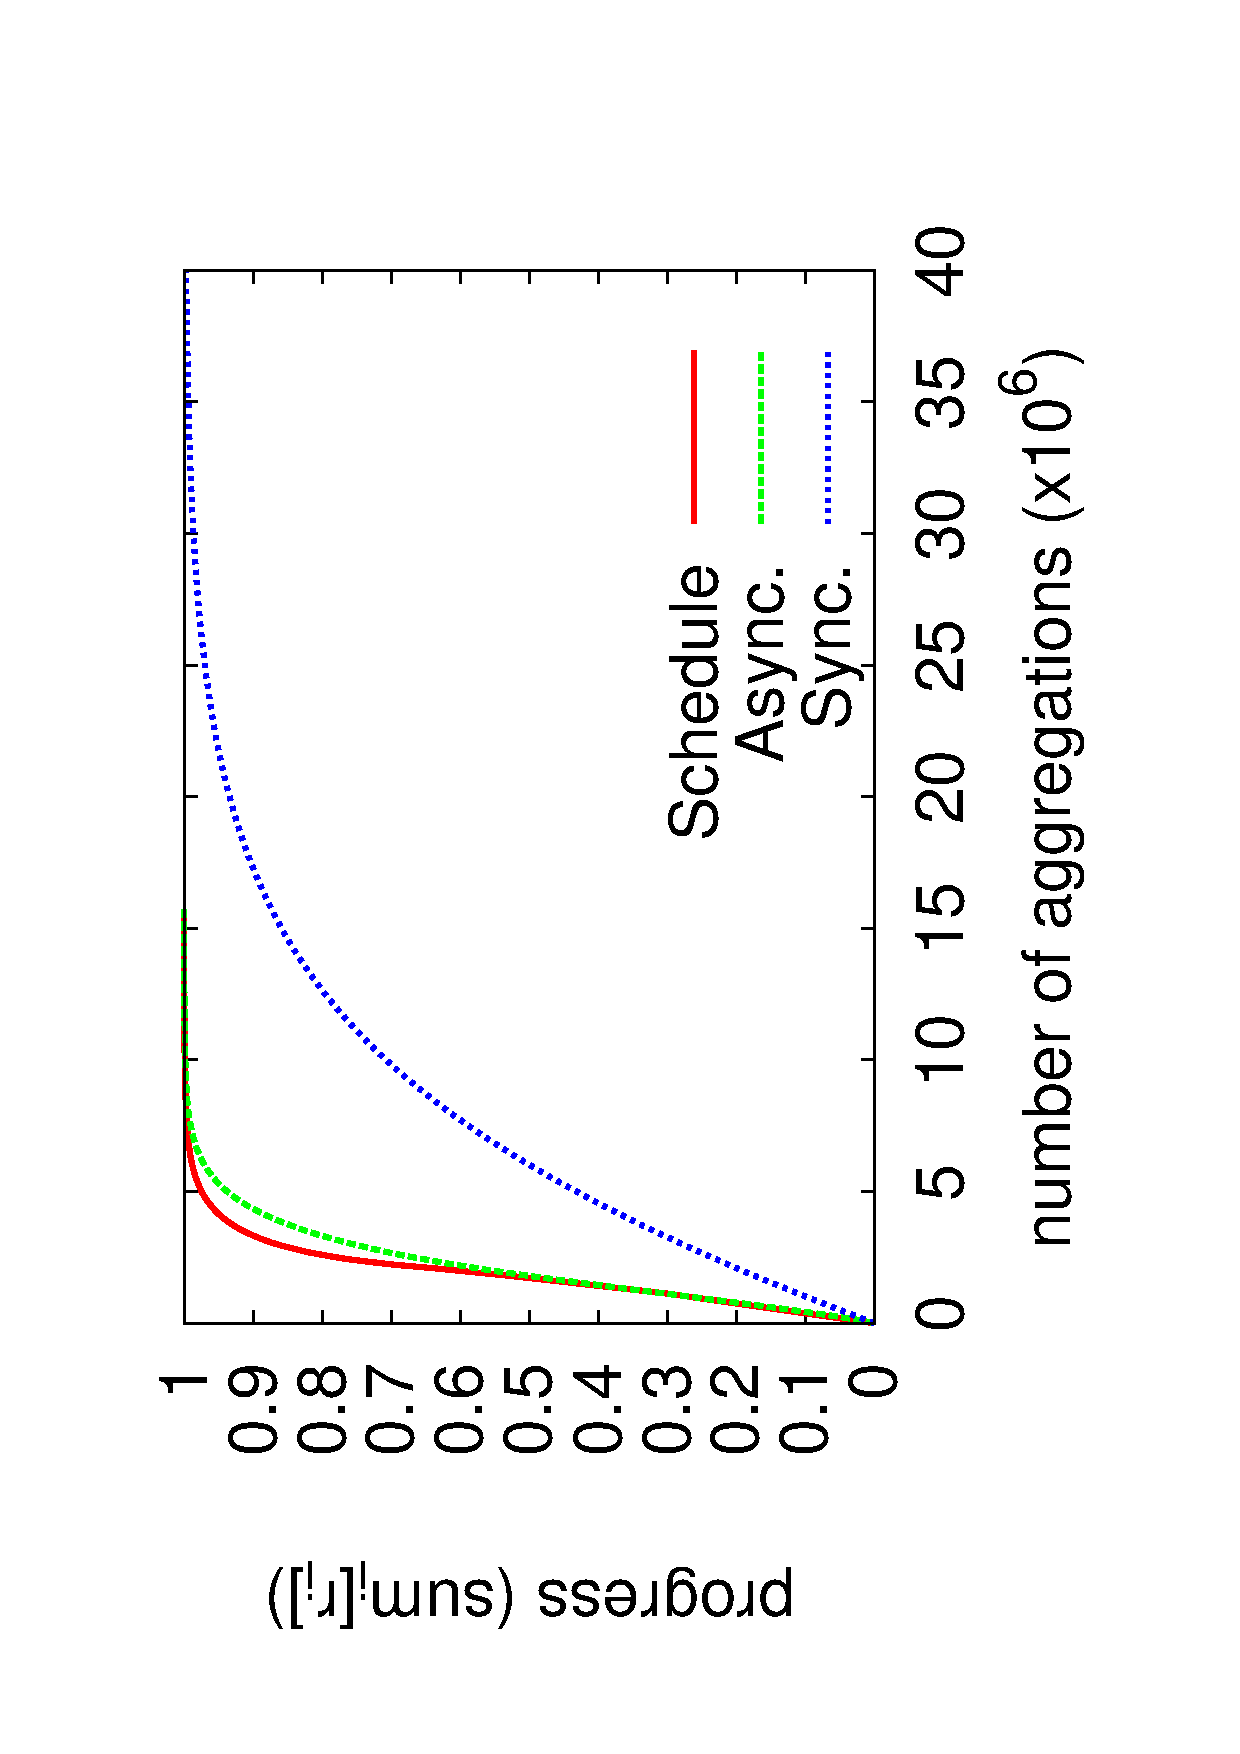
\includegraphics[width=1.3in, angle=-90]{fig/roadca_aggregate_progress}
 \label{fig:single-numagg:roadca}
 \vspace{-0.05in}}
 \hspace{-5mm}
 \subfloat[Livejournal]{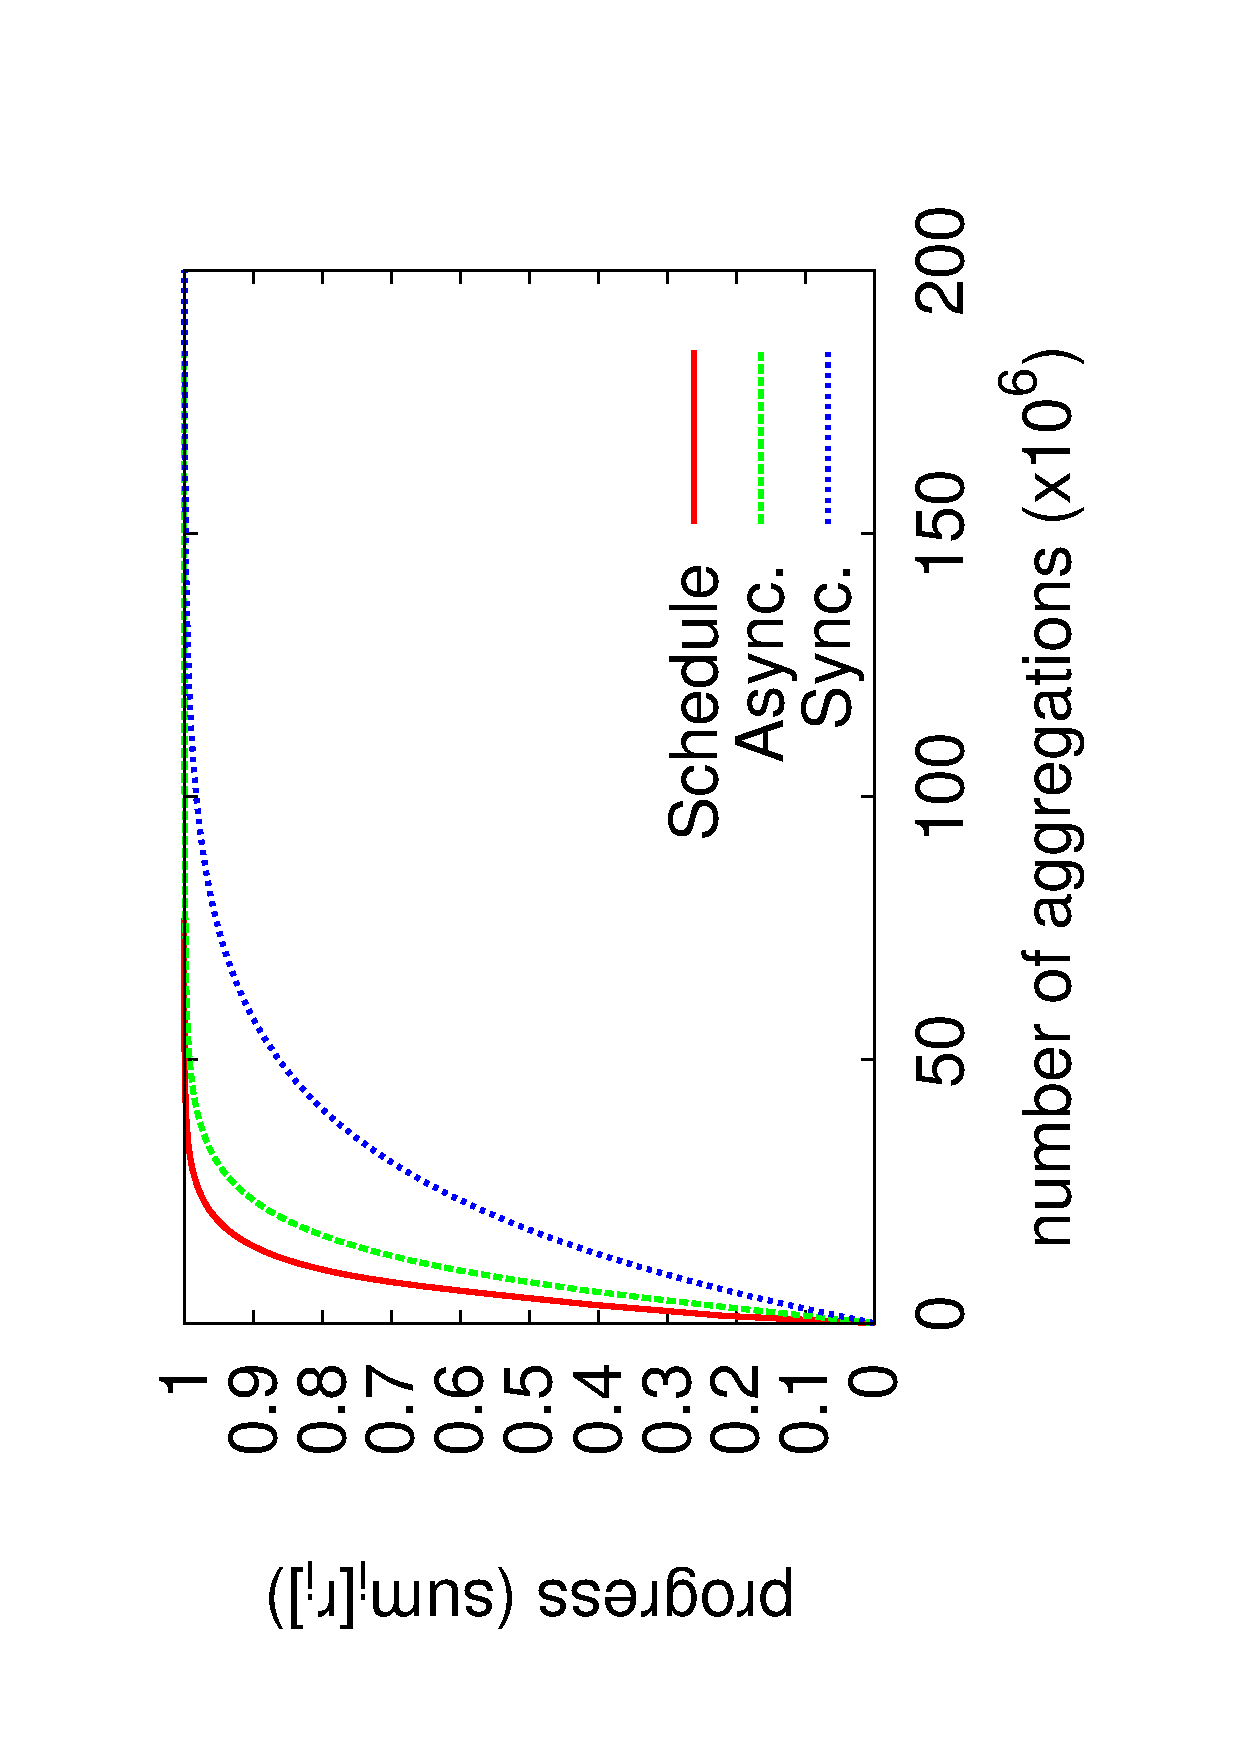
\includegraphics[width=1.3in, angle=-90]{fig/livejournal_aggregate_progress}
 \label{fig:single-numagg:livejournal}
 \vspace{-0.05in}}
 }
 \vspace{-0.1in}
 \caption{Effectiveness of aggregate operations to converging progress}
 \label{fig:single-numagg}
 \vspace{-0.1in}
 \end{figure}
In this experiment, we evaluate the effectiveness of asynchronous aggregations on accelerating the computation prog-ress.
 
 We run PageRank on two datasets, RoadCA and Livejournal, which result in the most speedup and the least speedup comparing to synchronous aggregation as shown in Table \ref{tab:wrokload}. We record the accumulated number of aggregate operations during the computation. In the accumulated version of PageRank (see Sec. \ref{sec:async:convert}), the summation of ranking scores $\sum_i{r_i}$ is approaching to 1 and will finally converge to 1. So we estimate the computation progress by evaluating $\sum_i{r_i}$ periodically. Fig. \ref{fig:single-numagg} shows the results. By using asynchronous aggregation, the converging progress is much faster than using synchronous execution. The scheduling of aggregate operations will further speedup the progress. The asynchronous aggregation with scheduling shows more effectiveness, so that each aggregate operation contributes more. It also shows more effectiveness on the RoadCA graph than on the Lievejournal graph. This is the reason why higher speedup is observed on the RoadCA graph.
\end{comment}
\end{appendix}




\end{document}
